\chapter{Infinite Sequences and Series}

\emph{Omitted from this excerpt}\endinput

% Begin Section 9.1
\section{Sequences and Series}
In the 5\textsuperscript{th} century B.C. the ancient Greek philosopher Zeno of
Elea\index{Zeno's motion paradox} devised several paradoxes, the most famous of
which---\emph{The Dichotomy}---asserts that if space is infinitely divisible
then motion is impossible. The argument goes like this: imagine a line segment
of finite length, say 1 m, with a person at one end as in
Figure \ref{fig:zeno}.\index{sequence}\index{series}

\begin{figure}[ht]
\centering
\begin{tikzpicture}[>=latex,every node/.style={font=\small}]
 \node at (-0.4,1) {
\includegraphics[scale=0.6]{zeno}};
 \draw[linecolor,line width=1.5,anchor=base] (0,0) -- (8,0)
  node[black,shift={(0,-0.5)}] at (0,0) {$0$}
  node[black,shift={(0,-0.5)}] at (0.5,0) {$\ldots$}
  node[black,shift={(0,-0.5)}] at (1,0) {$\frac{1}{8}$}
  node[black,shift={(0,-0.5)}] at (2,0) {$\frac{1}{4}$}
  node[black,shift={(0,-0.5)}] at (4,0) {$\frac{1}{2}$}
  node[black,shift={(0,-0.5)}] at (8,0) {$1$};
 \fill (0,0) circle (3pt);
 \fill (1,0) circle (2.5pt);
 \fill (2,0) circle (2.5pt);
 \fill (4,0) circle (2.5pt);
 \fill (8,0) circle (3pt);
\end{tikzpicture}
\caption[]{\enskip Zeno's motion paradox}
\label{fig:zeno}
\end{figure}

Before traversing the entire distance the person would first need to travel
one half the distance. Before doing that, though, he would need to travel one
fourth the distance, and before that one eighth the distance, and so on. There
is thus no ``first'' distance for him to traverse, meaning his motion cannot
even begin!

Obviously motion is possible, or you would not be reading this. Does that mean
Zeno's reasoning is flawed? More on that later. In the meantime, notice a
few things in Figure \ref{fig:zeno}. First, the distance markers
$\frac{1}{2},\frac{1}{4},\frac{1}{8},\ldots$ form an \textbf{infinite sequence}
of numbers approaching 0. Second, the sum of the distances between successive
markers is an \textbf{infinite series} which should equal the total segment
length 1:
\[
\frac{1}{2} ~+~ \frac{1}{4} ~+~ \frac{1}{8} ~+~ \cdots ~=~ 1
\]
It will be shown shortly that the sum is indeed 1, which turns out to have no
bearing on Zeno's paradox. First some definitions are needed.
\newpage
A \textbf{sequence} is an ordered list of objects, which in this book will
always be real numbers. Sequences can be finite or infinite:
finite if there is a last number in the list, infinite if every number in the
list is followed by another number (i.e. a ``successor''). Sequences should not
be confused with \emph{sets}---order matters in a sequence but not in a
set, and numbers may repeat in a sequence but not in a set.\index{sequence}

For example, the sequences $\langle 1,2,3\rangle$ and $\langle 1,3,2\rangle$ are
different, since order matters. However, the numbers in those sequences comprise
the same set $\lbrace 1,2,3\rbrace$.

The simplest example of an infinite sequence is $\Naturals$, the set
of natural numbers: $0,1,2,3,\ldots$. In fact, the numbers $a_0,a_1,a_2,\ldots$
in any infinite sequence of real numbers can be written as the range of a
function $f$ mapping $\Naturals$ into $\Reals$:
\begin{equation}\label{eqn:seqfcn}
f(n) ~=~ a_n
\end{equation}
Typically notation such as $\seq{a_n}_{n=0}^{\infty}$ is used for representing
an infinite sequence, or simply $\seq{a_n}$ when the initial value of the index
$n$ is understood (and $n$ is always an integer).
The intuitive notion of the \textbf{limit} of an infinite sequence can be stated
formally:\index{sequence!limit}

\statedefn{defn:seqlimit}{A real number $L$ is the \textbf{limit} of an infinite
sequence $\seq{a_n}$, written as
\[
\lim_{n \to \infty} a_n ~=~ L \quad\text{or simply}\quad a_n \,\rightarrow\, L ~,
\]
if for any given number $\epsilon > 0$ there exists an integer $N$ such that
\begin{equation}\label{eqn:seqlimit}
\Abs{a_n - L} < \epsilon \quad\text{for all $n > N~$.}
\end{equation}
In this case the sequence $\seq{a_n}$ is said to \textbf{converge} to $L$ and is
called a \textbf{convergent sequence}. A sequence that is not convergent is
\textbf{divergent}.\index{sequence!convergent}\index{sequence!divergent}}

In other words, a sequence $\seq{a_n}$ converges to $L$ if the terms $a_n$ can
be made arbitrarily close to $L$ for $n$ sufficiently large. In most cases the
formal definition will not be needed, since by formula (\ref{eqn:seqfcn}) the
same rules and formulas from Chapters 1 and 3 for the limit of a function $f(x)$
as $x$ approaches $\infty$ apply to sequences (e.g. sums and products of limits,
L'H\^{o}pital's Rule). All you have to do is replace $x$ by $n$.

\begin{exmp}
\noindent For integers $n \ge 1$ define $a_n = \frac{1}{2^n}$. Find
$\displaystyle\lim_{n \to \infty} a_n$ if it exists.\vspace{1mm}
\par\noindent\emph{Solution:} Since
$\displaystyle\lim_{x \to \infty} \,\frac{1}{2^x} = 0$ then replacing $x$ by $n$
shows that
\[
\lim_{n \to \infty} a_n ~=~ \lim_{n \to \infty}~ \frac{1}{2^n} ~=~ 0 ~.
\]
\end{exmp}
\divider
\newpage
\begin{exmp}
\noindent For integers $n \ge 0$ define $a_n = \frac{2n+1}{3n+2}$. Is
$\seq{a_n}$ a convergent sequence? If so then find its limit.\vspace{1mm}
\par\noindent\emph{Solution:} By L'H\^{o}pital's Rule, treating an integer
$n\ge 0$ as a real-valued variable $x$,
\[
\lim_{n \to \infty} a_n ~=~ \lim_{n \to \infty}~ \frac{2n+1}{3n+2} ~=~ 
\lim_{n \to \infty}~ \frac{2}{3} ~=~ \frac{2}{3} ~.
\]
Thus the sequence is convergent and its limit is $\frac{2}{3}$.
\end{exmp}
\begin{exmp}
\noindent For integers $n \ge 0$ define $a_n = \frac{e^n}{3n+2}$. Is
$\seq{a_n}$ a convergent sequence? If so then find its limit.\vspace{1mm}
\par\noindent\emph{Solution:} By L'H\^{o}pital's Rule, treating an integer
$n\ge 0$ as a real-valued variable $x$,
\[
\lim_{n \to \infty} a_n ~=~ \lim_{n \to \infty}~ \frac{e^n}{3n+2} ~=~
\lim_{n \to \infty}~ \frac{e^n}{3} ~=~ \infty
\]
Thus the sequence is divergent.\index{recurrence relation}
\end{exmp}
\begin{exmp}\label{exmp:fib}
\noindent The famous \emph{Fibonacci sequence}\footnote{Due to the Italian
mathematician Leonardo Fibonacci (ca. 1170-1250).} $\seq{F_n}$ starts with the
numbers 0 and 1, then each successive term is the sum of the previous two
terms: $F_0 = 0$, $F_1 = 1$,\index{Fibonacci sequence}
\begin{equation}\label{eqn:fibonacci}
F_n ~=~ F_{n-1} ~+~ F_{n-2} ~~\text{for integers $n \ge 2$}
\end{equation}
Equation (\ref{eqn:fibonacci}) is a \emph{recurrence relation}.
The first ten Fibonacci numbers are $0,1,1,2,3,5,8,13,21,34$. Clearly
$\seq{F_n}$ is a divergent sequence, since $F_n \rightarrow \infty$. For
$n \ge 2$ define $a_n = F_n/F_{n-1}$. The first few values are:
\[
a_2 ~=~ \frac{F_2}{F_1} ~=~ \frac{1}{1} ~=~ 1 \quad,\quad
a_3 ~=~ \frac{F_3}{F_2} ~=~ \frac{2}{1} ~=~ 2 \quad,\quad
a_4 ~=~ \frac{F_4}{F_3} ~=~ \frac{3}{2} ~=~ 1.5 \quad,\quad
a_5 ~=~ \frac{F_5}{F_4} ~=~ \frac{5}{3} ~\approx~ 1.667
\]
Show that $\seq{a_n}$ is
convergent. In other words, in the Fibonacci sequence the ratios of each term to
the previous term converge to some number.\index{sequence!Fibonacci}\vspace{1mm}
\par\noindent\emph{Solution:} There are many ways to prove this, perhaps the
simplest being to assume the sequence is convergent and then find the limit
(which would be impossible if the sequence were divergent). So assume that
$a_n \rightarrow a$ for some real number $a$. Then divide both sides of
formula (\ref{eqn:fibonacci}) by $F_{n-1}$, so that
\[
\frac{F_n}{F_{n-1}} ~=~ 1 ~+~ \frac{F_{n-2}}{F_{n-1}} \quad\Rightarrow\quad
a_n ~=~ 1 ~+~ \frac{1}{a_{n-1}} ~~\text{for integers $n \ge 2$}
\]
Now take the limit of both sides of the last equation as $n \to \infty$:
\[
\lim_{n \to \infty} ~a_n ~=~ \lim_{n \to \infty} ~\left(1 ~+~ \frac{1}{a_{n-1}}\right)
\quad\Rightarrow\quad
a ~=~ 1 ~+~ \frac{1}{a} \quad\Rightarrow\quad a^2 - a - 1 ~=~ 0
\quad\Rightarrow\quad
a ~=~ \frac{1 \pm \sqrt{5}}{2}
\]
Since $a$ must be positive then $a = \frac{1 +\sqrt{5}}{2}$. Thus, the sequence
is convergent and converges to $\frac{1 +\sqrt{5}}{2} \approx 1.618$. \\Note:
This number is the famous \emph{golden ratio}, the subject of many claims
regarding its appearance in nature and supposed aesthetic appeal as a ratio of
sides of a rectangle.\footnote{For example, see \textsc{Huntley, H.E.},
\emph{The Divine Proportion}, New York: Dover Publications, Inc.,
1970.}\index{golden ratio}
\end{exmp}
\divider
\newpage
An \textbf{infinite series}\index{infinite series} is the sum of an infinite
sequence. If the infinite sequence is $\seq{a_n}_{n=0}^{\infty}$ then the series
can be written as\index{series!infinite}\index{infinite series!sum}
\[
\sum_{n=0}^{\infty} a_n ~=~ a_0 + a_1 + a_2 + \cdots + a_n + \cdots
\]
or simply as $\sum a_n$ when the initial value of the index $n$ is understood.
There is a natural way to define the sum of such a series:

\statedefn{defn:sumofseries}{The \textbf{sum} of an infinite series
$\displaystyle\sum_{n=0}^{\infty} a_n$ is
\begin{equation}\label{eqn:sumofseries}
\sum_{n=0}^{\infty} a_n ~=~ \lim_{n \to \infty} ~s_n
\end{equation}
where $\seq{s_n}_{n=0}^{\infty}$ is the sequence of \textbf{partial sums} of the
series:\index{infinite series!partial sum}\index{infinite series!divergent}
\[
s_n ~=~ \sum_{k=0}^n a_k ~=~ a_0 + a_1 + a_2 + \cdots + a_n \quad\text{for $n\ge 0$}
\]
If the partial sums $\seq{s_n}$ converge to a real number $s$ then the series is
\textbf{convergent}, and \textbf{converges} to $s$; if $\seq{s_n}$ diverges then
the series is \textbf{divergent}.\index{infinite series!convergent}}

One important convergent series is a \textbf{geometric progression}:
\begin{equation}\label{eqn:geomprog}
a + ar + ar^2 + ar^3 + \cdots + ar^n + \cdots
\end{equation}
with $a \ne 0$ and $\abs{r} < 1$. Multiply the $n$-th partial sum $s_n$ by $r$:
\[
rs_n ~=~ r\,(a + ar + ar^2 + ar^3 + \cdots + ar^{n-1} + ar^n) ~=~
ar + ar^2 + ar^3 + ar^4 + \cdots + ar^n + ar^{n+1}
\]
Now subtract $rs_n$ from $s_n$:
\begin{align*}
s_n - rs_n ~&=~ a + ar + ar^2 + ar^3 + \cdots + ar^n -
               (ar + ar^2 + ar^3 + ar^4 + \cdots + ar^n + ar^{n+1})\\
s_n - rs_n ~&=~ a - ar^{n+1} \quad\text{so that}\\
\lim_{n \to \infty} s_n ~&=~ \lim_{n \to \infty} \frac{a\,(1 - r^{n+1})}{1 -r} ~=~ \frac{a}{1-r}
\end{align*}
since $r^{n+1} \rightarrow 0$ as $n \to \infty$ when $\abs{r} < 1$. Thus:

\statethm{thm:geomprogsum}{For $a \ne 0$ and $\abs{r} < 1$ the geometric
progression $\displaystyle\sum_{n=0}^{\infty} ar^n$ is convergent:\vspace{-2mm}
\begin{equation}\label{eqn:geomprogsum}
\sum_{n=0}^{\infty} ar^n ~=~ a + ar + ar^2 + ar^3 + \cdots + ar^n + \cdots ~=~ \frac{a}{1-r}
\end{equation}}
\newpage
\begin{exmp}\label{exmp:geomzeno}
\noindent Show that
$\displaystyle\sum_{n=1}^{\infty} \,\frac{1}{2^n} = 1$.\vspace{1mm}
\par\noindent\emph{Solution:} This is a geometric progression with
$a=\frac{1}{2}$ and $r=\frac{1}{2}$. So by formula (\ref{eqn:geomprogsum}) the
sum is:
\[
\sum_{n=1}^{\infty} \;\frac{1}{2^n} ~=~
\sum_{n=0}^{\infty} \;\left(\frac{1}{2}\right) \,\cdot\, \left(\frac{1}{2}\right)^n ~=~ \frac{a}{1-r} ~=~
\frac{\frac{1}{2}}{1 - \frac{1}{2}} ~=~ 1 \quad\checkmark
\]
\end{exmp}
\begin{exmp}
\noindent Write the repeating decimal $0.\overline{17} = 0.17171717\ldots$ as a
rational number.\vspace{1mm}
\par\noindent\emph{Solution:} This is a geometric progression with
$a=0.17=\frac{17}{100}$ and $r=0.01=\frac{1}{100}$:
\begin{align*}
0.171717\ldots ~&=~ 0.17 + 0.0017 + 0.000017 + \cdots
~=~ 0.17\,(0.01)^0 + 0.17\,(0.01)^1 + 0.17\,(0.01)^2 + \cdots\\
&=~ \sum_{n=0}^{\infty} \;0.17\,(0.01)^n  ~=~ \frac{a}{1-r} ~=~
\frac{0.17}{1 - 0.01} ~=~ \frac{0.17}{0.99} ~=~ \frac{17}{99}
\end{align*}
\end{exmp}
\divider
\vspace{2mm}

Back to Zeno's motion paradox, by Example \ref{exmp:geomzeno} the sum of the
infinite number of distances between successive markers in Figure \ref{fig:zeno}
is 1, as expected. This fact is often mistaken as proof that Zeno was wrong, yet
it does not actually address Zeno's argument, since the person is attempting to
begin motion at the tail end---the ``infinite end''---of the geometric
progression, not at the beginning (i.e. at $n=0$). Zeno's point remains that
there is no ``first step'' at that tail end.\index{Zeno's motion paradox}

In fact, even if you were to reverse the person's position to start at the other
end, so that he would first move a distance $\frac{1}{2}$, then a distance
$\frac{1}{4}$, and so on, as in Figure \ref{fig:zenoreverse}, then a new problem
is introduced: the person keeps moving no matter how close he is to the end
point. There is now no ``last step'' and motion is thus still impossible.

\begin{figure}[ht]
\centering
\begin{tikzpicture}[>=latex,every node/.style={font=\small}]
 \node[xscale=-1] at (8.4,1) {
\includegraphics[scale=0.6]{zeno}};
 \draw[linecolor,line width=1.5,anchor=base] (0,0) -- (8,0)
  node[black,shift={(0,-0.5)}] at (0,0) {$0$}
  node[black,shift={(0,-0.5)}] at (0.5,0) {$\ldots$}
  node[black,shift={(0,-0.5)}] at (1,0) {$\frac{1}{8}$}
  node[black,shift={(0,-0.5)}] at (2,0) {$\frac{1}{4}$}
  node[black,shift={(0,-0.5)}] at (4,0) {$\frac{1}{2}$}
  node[black,shift={(0,-0.5)}] at (8,0) {$1$};
 \fill (0,0) circle (3pt);
 \fill (1,0) circle (2.5pt);
 \fill (2,0) circle (2.5pt);
 \fill (4,0) circle (2.5pt);
 \fill (8,0) circle (3pt);
 \draw[decorate,decoration={brace,raise=7pt,amplitude=5pt}] (4,0) -- (8,0)
  node[midway,above,yshift=5mm] {$\frac{1}{2}$};
 \draw[decorate,decoration={brace,raise=7pt,amplitude=5pt}] (2,0) -- (4,0)
  node[midway,above,yshift=5mm] {$\frac{1}{4}$};
 \draw[decorate,decoration={brace,raise=7pt,amplitude=5pt}] (1,0) -- (2,0)
  node[midway,above,yshift=5mm] {$\frac{1}{8}$};
 \node[above] at (0.5,0.2) {$\cdots$};
\end{tikzpicture}
\caption[]{\enskip Zeno's motion paradox in reverse}
\label{fig:zenoreverse}
\end{figure}

The convergence of the geometric progression has misled many people to argue
that Zeno is wrong, by claiming it shows an infinite number of movements
can be completed in a finite amount of time. But this line of argument fails on
(at least) two counts. First, Zeno never argued about time---it is irrelevant to
his paradox. The more fundamental flaw is that the introduction of time brings
along the concept of speed, typically taken to be constant (though it need not
be). Speed is distance over time, but it is precisely the \emph{distance} part
of that ratio that Zeno rejects---that distance can never be traveled. In other
words, it is circular---and hence faulty---reasoning to ``prove'' that motion is
possible by \emph{assuming} it is possible.

The geometric progression also doesn't help when considering only the
distances and ignoring time. Even assuming each of those distances could be
traveled, the partial sums
\emph{approach} 1 but never actually \emph{reach} it. The limit of a
sequence is defined in terms of an inequality---you can get arbitrarily
close to the limit, and that is all. The equality in formula
(\ref{eqn:geomprogsum}) is merely a shorthand way of saying that. It is an
abstraction based on properties of the real number system, not necessarily
based on physical reality.

Zeno's paradox is not purely mathematical---it is about space and hence is
physical, with a tinge of philosophy. Physicists have recognized this---and
noted the flaw in the purely mathematical line of attack---and devised new
arguments against Zeno, some more sophisticated than others. However, they
all invariably end up in some sort of circular reasoning.
All this calls into question the original assumption: the infinite divisibility
of space. If space had some smallest unit that could not be divided any further
then there is no paradox---motion over a finite distance could always be
decomposed into a large but finite number of irreducible steps.\footnote{As of
this writing there is not yet a
definitive answer as to whether space is continuous or discrete (quantized).
A ``smallest unit'' would have to be below the \emph{Planck level}---around
$10^{-33}$ cm, well below current measurement capabilities. Some recent advances
in the field of \emph{loop quantum gravity} suggest the possibility of quantized
space. See \textsc{Chamseddine, A.H., Connes, A. \& Mukhanov, V.}, ``Geometry and
the quantum: basics.'' \emph{J. High Energy Phys.} \textbf{2014}, 98 (2014).
 \url{https://doi.org/10.1007/JHEP12(2014)098}}\vspace{1mm}

\divider
\vspace{2mm}
\startexercises\label{sec9dot1}
{\small
\probs{A}
\par\noindent For Exercises 1-8, determine if the given sequence is
convergent. If so then find its limit.
\begin{enumerate}[item-label={\bfseries \arabic*.}]
\begin{multicols}{4}
 \item $\seq{n\,e^{-n}}_{n = 0}^{\infty}\vphantom{\seq{\dfrac{n^2}{3n^2 ~+~ 7n ~-~ 2}}_{n = 1}^{\infty}}$
 \item $\seq{\dfrac{n^2}{3n^2 ~+~ 7n ~-~ 2}}_{n = 1}^{\infty}$
 \item $\seq{\dfrac{n^2}{3n^3 ~+~ 7n ~-~ 2}}_{n = 1}^{\infty}$
 \item $\seq{\dfrac{n^3}{3n^2 ~+~ 7n ~-~ 2}}_{n = 1}^{\infty}$
\end{multicols}
\begin{multicols}{4}
 \item $\seq{\dfrac{n}{\ln\,n}}_{n = 2}^{\infty}\vphantom{\seq{\dfrac{n\,!}{(n + 2)\,!}}_{n = 0}^{\infty}}$
 \item $\seq{\dfrac{n\,!}{(n + 2)\,!}}_{n = 0}^{\infty}$
 \item $\seq{\sin\,\left(\dfrac{n \pi}{2}\right)}_{n = 0}^{\infty}\vphantom{\seq{\dfrac{n\,!}{(n + 2)\,!}}_{n = 0}^{\infty}}$
 \item $\seq{(-1)^n \cos\,n\pi}_{n = 0}^{\infty}\vphantom{\seq{\dfrac{n\,!}{(n + 2)\,!}}_{n = 0}^{\infty}}$
\end{multicols}
\suspend{enumerate}
\par\noindent For Exercises 9-12 determine whether the given series is
convergent. If so then find its sum.

\begin{multicols}{4}
\resume{enumerate}[item-label={{[\bfseries \arabic*.]}}]
 \item $\bigsum{n = 0}{\infty}~ 2\;\left(\dfrac{2}{3}\right)^n$
 \item $\bigsum{n = 1}{\infty}~ 7^{-n}$
 \item $\bigsum{n = 0}{\infty}~ \dfrac{3^n ~+~ 5^{n + 1}}{6^n}$
 \item $\bigsum{n = 0}{\infty}~ n$
\suspend{enumerate}
\end{multicols}
\par\noindent For Exercises 13-16 use a geometric progression to write the given
repeating decimal as a rational number.
\resume{enumerate}[item-label={{[\bfseries \arabic*.]}}]
\begin{multicols}{4}
 \item $0.\overline{113}$
 \item $0.\overline{9}$
 \item $0.24\overline{9}$
 \item $0.01\overline{7}$
\end{multicols}
\suspend{enumerate}
\probs{B}
\resume{enumerate}[item-label={{[\bfseries \arabic*.]}}]
 \item In Example \ref{exmp:fib} define $b_n = F_n/F_{n+1}$ for $n\ge 0$ and
 show that $\seq{b_n}_{n=0}^{\infty}$ converges to $\frac{\sqrt{5}-1}{2}$.
 \item Show that formula (\ref{eqn:newton}) for Newton's method with
 $f(x) = x^2 - 2$ and $x_0 = 1$ yields the sequence $\seq{x_n}_{n=0}^{\infty}$
 with
\[
x_n ~=~ \frac{1}{2} x_{n-1} ~+~ \frac{1}{x_{n-1}} \quad\text{for $n\ge 1\;$,}
\]
then assuming $\seq{x_n}$ is convergent show that it must converge to
$\sqrt{2}$. \emph{(Hint: See Example \ref{exmp:fib}.)}
 \item In this exercise you will prove a formula for the general number $F_n$
  in the Fibonacci sequence. Denote the positive and negative solutions to the
  equation $x^2 - x - 1 = 0$ by $\phi_{+} = \frac{1+\sqrt{5}}{2}$ and
  $\phi_{-} = \frac{1-\sqrt{5}}{2}$, respectively. Note that $\phi_{+}$ is the
  golden ratio mentioned in Example \ref{exmp:fib}.
\begin{enumerate}[item-label={\bfseries (\alph*)}]
 \item Use the equation $x^2 - x - 1 = 0$ to show that
\[
\phi_{+}^{n+1} ~=~ \phi_{+}^{n} ~+~ \phi_{+}^{n-1} \qquad\text{and}\qquad
\phi_{-}^{n+1} ~=~ \phi_{-}^{n} ~+~ \phi_{-}^{n-1} ~.
\]
 \item Use part (a) and induction to show that\index{Fibonacci sequence}
\[
F_n ~=~ \frac{\phi_{+}^{n} \;-\; \phi_{-}^{n}}{\sqrt{5}} \quad\text{for $n\ge 0$.}
\]
\end{enumerate}
 \item A ball is dropped from a height of 4 ft above the ground, and upon
  each bounce off the ground the ball bounces straight up to a height equal to
  65\% of its previous height. Find the theoretical total distance the ball
  could travel if it could bounce indefinitely. Why is this physically
  unrealistic?
 \item A \emph{continued fraction}\index{continued fraction} is a type of
  infinite sum involving a fraction with a denominator that continues
  indefinitely:
\[
a ~=~ a_0 ~+~ \cfrac{1}{a_1 \;+\; \cfrac{1}{a_2 \;+\; \cfrac{1}{a_3 \;+\; \cdots}}}
\]
\begin{enumerate}[item-label={\bfseries (\alph*)}]
 \item Show that the golden ratio $\phi_{+} = \frac{1+\sqrt{5}}{2}$ (a solution of
 $x^2-x-1=0$) can be written as\index{golden ratio}
\[
\phi_{+} ~=~ 1 ~+~ \cfrac{1}{1 \;+\; \cfrac{1}{1 \;+\; \cfrac{1}{1 \;+\; \cdots}}} ~.
\]
\emph{(Hint: Look for a recurrence relation in the fraction.)}
 \item Show that
\[
\sqrt{2} ~=~ 1 ~+~ \cfrac{1}{2 \;+\; \cfrac{1}{2 \;+\; \cfrac{1}{2 \;+\; \cdots}}} ~.
\]
\end{enumerate}
 \item\label{exer:goldensqrt} Show that the golden ratio
  $\phi_{+} = \frac{1+\sqrt{5}}{2}$ can be written as
  $\phi_{+} = \sqrt{1 + \sqrt{1 + \sqrt{1 + \cdots}}}$.
 \item Write a computer program to approximate the result in Exercise
  \ref{exer:goldensqrt} using $100$ terms. After how many iterations do the
   approximate values start repeating?
 \item Would the existence of infinitesimals as a measure of space resolve
  Zeno's paradox? Explain.
\end{enumerate}
}
\newpage
%Begin Section 9.2
\section{Tests for Convergence}
There are many ways to determine if a sequence converges---two are
listed below. In all cases changing or removing a finite number of terms in a
sequence does not affect its convergence or divergence:\index{Comparison Test}

\statethm{thm:seqtests}{\begin{enumerate}[item-label={\bfseries \arabic*.}]
\item \textbf{Monotone Bounded Test}: A sequence that is bounded and
\emph{monotone}---i.e. either always increasing or always decreasing---is
convergent.\index{sequence!Monotone Bounded Test}\index{Monotone Bounded Test}
\item \textbf{Comparison Test}: If $\seq{b_n}$ diverges to $\infty$ and if
$\seq{a_n}$ is a sequence such that $a_n \ge b_n$ for all $n > N$ for some $N$,
then $\seq{a_n}$ also diverges to $\infty$.\\Likewise, if $\seq{c_n}$ diverges
to $-\infty$ and $a_n \le c_n$ for all $n > N$ for some $N$, then $\seq{a_n}$
also diverges to $-\infty$.\index{sequence!Comparison Test}
\end{enumerate}}

\piccaption[]{\label{fig:mbtest}}\parpic[r]{
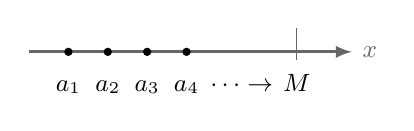
\begin{tikzpicture}[>=latex,every node/.style={font=\small}]
 \draw[->,black!60,line width=1pt,anchor=base] (0,0) -- (4.1,0) node[right] {$x$}
  node[black,shift={(0,-0.5)}] at (0.5,0) {$a_1$}
  node[black,shift={(0,-0.5)}] at (1,0) {$a_2$}
  node[black,shift={(0,-0.5)}] at (1.5,0) {$a_3$}
  node[black,shift={(0,-0.5)}] at (2,0) {$a_4$}
  node[black,shift={(0,-0.5)}] at (2.7,0) {$\cdots \rightarrow$}
  node[black,shift={(0,-0.5)}] at (3.4,0) {$M$};
 \fill (0.5,0) circle (1.5pt);
 \fill (1,0) circle (1.5pt);
 \fill (1.5,0) circle (1.5pt);
 \fill (2,0) circle (1.5pt);
 \draw[black!60] (3.4,0.3) -- (3.4,-0.1);
\end{tikzpicture}}
\noindent The Comparison Test makes sense intuitively, since something larger
than a quantity going to infinity must also go to infinity. The Monotone Bounded
Test can be understood by thinking of a bound on a sequence as a wall that the
sequence can never pass, as in Figure \ref{fig:mbtest}. The increasing sequence
$\seq{a_n}$ in the figure moves toward $M$ but can never pass it. The sequence
thus cannot diverge to
$\infty$, and it cannot fluctuate back and forth since it always increases. Thus
it must converge somewhere before or at $M$.\footnote{For a proof see pp.48-49
in \textsc{Buck, R.C.}, \emph{Advanced Calculus}, 2nd ed., New York: McGraw-Hill
Book Co., 1965.} Notice that the Monotone Bounded Test tells you only that the
sequence converges, not what it converges to.

\begin{exmp}
\noindent Show that the sequence $\seq{a_n}_{n=1}^{\infty}$ defined for $n\ge 1$
by
\[
a_n ~=~ \frac{1 \,\cdot\, 3 \,\cdot\, 5 \,\cdots\, (2n-1)}
{2 \,\cdot\, 4 \,\cdot\, 6 \,\cdots\, (2n)}
\]
is convergent.\vspace{1mm}
\par\noindent\emph{Solution:} Notice that $\seq{a_n}$ is always decreasing,
since
\[
a_{n+1} ~=~ \frac{1 \,\cdot\, 3 \,\cdot\, 5 \,\cdots\, (2n-1) \,\cdot\, (2n+1)}
{2 \,\cdot\, 4 \,\cdot\, 6 \,\cdots\, (2n)\,\cdot\, (2n+2)} ~=~
a_n \,\cdot\, \frac{2n+1}{2n+2} ~<~ a_n \,\cdot\, (1) ~=~ a_n
\]
for $n\ge 1$. The sequence is also bounded, since $0 < a_n$ and
\[
a_n ~=~ \frac{1}{2} \,\cdot\, \frac{3}{4} \,\cdot\, \frac{5}{6} \,\cdots\,
\frac{2n-1}{2n} ~<~ 1 \quad\text{for $n\ge 1$}
\]
since each fraction in the above product is less than 1. Thus, by the Monotone
Bounded Test the sequence is convergent.\\Note that for a decreasing sequence
only the lower bound is needed for the Monotone Bounded Test, not the upper
bound. Similarly, for an increasing sequence only the upper bound matters.
\end{exmp}
\divider
\newpage
\noindent Some tests for convergence of a series are listed below:

\statethm{thm:seriestests}{\begin{enumerate}[item-label={\bfseries \arabic*.}]
\item \textbf{n-th Term Test}: If\index{series!n-th Term Test}
$\sum a_n$ converges then $\displaystyle\lim_{n \to \infty} a_n = 0$.
\item \textbf{Ratio Test}: For a series $\sum a_n$ of positive terms let
\[
R ~=~ \lim_{n \to \infty} \;\frac{a_{n+1}}{a_n} ~.
\]
Then\index{Ratio Test}\index{series!Ratio Test}
\begin{enumerate}[item-label={\bfseries (\alph*)}]
\item if $R < 1$ then the series converges,
\item if $R > 1$ (including $R = \infty$) then the series diverges,
\item if $R=1$ then the test fails.
\end{enumerate}
\item \textbf{Integral Test}: For a series\index{Integral Test}
$\displaystyle\sum_{n=1}^{\infty} a_n$ of positive terms let $f(x)$ be a
decreasing function on $\lival{1}{\infty}$ such that $f(n)=a_n$ for all integers
$n\ge 1$. Then\index{series!Integral Test}
\[
\sum_{n=1}^{\infty} a_n \quad\text{and}\quad \int_1^{\infty} f(x)~\dx
\]
either both converge or both diverge.
\item \textbf{p-series Test}: The series\index{p-series Test}
$\displaystyle\sum_{n=1}^{\infty} \frac{1}{n^p}$ converges for $p>1$, and
diverges for $p \le 1$.\index{series!p-series Test}
\item \textbf{Comparison Test}: If $0 \le a_n \le b_n$ for $n > N$ for some $N$,
and if $\sum b_n$ is convergent then $\sum a_n$ is convergent. Similarly, if
$0 \le b_n \le a_n$ for $n > N$ for some $N$, and if $\sum b_n$ is divergent
then $\sum a_n$ is divergent.\index{$n$-th Term Test}
\item \textbf{Limit Comparison Test}: For two series $\sum a_n$ and $\sum b_n$
of positive terms let\index{Limit Comparison Test}
\[
L ~=~ \lim_{n \to \infty} \;\frac{a_n}{b_n} ~.
\]
Then\index{series!Limit Comparison Test}
\begin{enumerate}[item-label={\bfseries (\alph*)}]
\item if $0 < L < \infty$ then $\sum a_n$ and $\sum b_n$ either both converge or
both diverge,\index{series!Telescoping Series Test}
\item if $L = 0$ and $\sum b_n$ converges then $\sum a_n$ converges,
\item if $L=\infty$ and $\sum b_n$ diverges then $\sum a_n$ diverges.
\end{enumerate}
\item \textbf{Telescoping Series Test}: Suppose\index{Telescoping Series Test}
$\sum a_n = \sum (b_n - b_{n+1})$ for some sequence $\seq{b_n}$. Then
$\sum a_n$ converges if and only if $b_n \rightarrow L$, in which case
$\sum a_n = b_1 - L$.
\end{enumerate}}
\newpage
Most of the above tests have fairly short proofs or at least
intuitive explanations. For example, the n-th Term Test follows from the
definition of convergence of a series: if $\sum a_n$ converges to a number $L$
then since each term $a_n = s_n - s_{n-1}$ is the difference of successive
partial sums, taking the limit yields
\[
\lim_{n \to \infty} \,a_n ~=~ \lim_{n \to \infty} \,(s_n - s_{n-1}) ~=~ L - L ~=~ 0
\]
by definition of the convergence of a series. $~\checkmark$\\Since the n-th
Term Test can never be used to prove convergence of a series, it is often stated
in the following logically equivalent manner:

\statethm{thm:nthtermtestdiv}{\textbf{n-th Term Test}: If
$\displaystyle\lim_{n \to \infty} a_n \ne 0$ then $\sum a_n$ diverges.}

\begin{exmp}
\noindent Show that $~\displaystyle\sum_{n=1}^{\infty} \,\dfrac{n}{2n+1} ~=~
\dfrac{1}{3} + \dfrac{2}{5} + \dfrac{3}{7} + \cdots~$ is
divergent.\vspace{1mm}
\par\noindent\emph{Solution:} Since
\[
\lim_{n \to \infty} \;\frac{n}{2n+1} ~=~ \frac{1}{2} ~\ne ~ 0
\]
then by the n-th Term Test the series diverges.
\end{exmp}
\divider
\vspace{2mm}

The Ratio Test takes a bit more effort to
prove.\footnote{See pp.612-613 in \textsc{Taylor, A.E. and W.R. Mann},
\emph{Advanced Calculus}, 2nd ed., New York: John Wiley \& Sons, Inc., 1972.}
When the ratio $R$ in the Ratio Test is larger than 1 then that means the terms
in the series do not approach 0, and thus the series diverges by the n-th Term
Test. When $R=1$ the test fails, meaning it is inconclusive---another test would
need to be used. When the test shows convergence it does not tell you what the
series converges to, merely that it converges.

\begin{exmp}
\noindent Determine if $~\displaystyle\sum_{n=1}^{\infty} \,\dfrac{n}{2^n}~$ is
convergent.\vspace{1mm}
\par\noindent\emph{Solution:} For the series general term $a_n = \frac{n}{2^n}$,
\[
R ~=~ \lim_{n \to \infty} \;\frac{a_{n+1}}{a_n} ~=~
\lim_{n \to \infty} \;\dfrac{\dfrac{n+1}{2^{n+1}}}{\dfrac{n}{2^n}} ~=~
\lim_{n \to \infty} \;\dfrac{n+1}{2n} ~=~ \frac{1}{2} ~<~ 1 ~,
\]
so by the Ratio Test the series converges.
\end{exmp}
\divider
\newpage
Figure \ref{fig:integraltest} shows why the Integral Test works.

\begin{figure}[ht]
\centering
\subfloat[][\enskip $\displaystyle\int_1^{\infty} f(x)\;\dx ~>~ \displaystyle\sum_{n=2}^{\infty} a_n$]{
\begin{tikzpicture}[>=latex,every node/.style={font=\small}]
 \draw[linecolor,line width=1.5pt,domain=1:5.5,samples=300] plot (\x, {2/\x});
 \draw (0,2) -- (1,2) -- (1,0) node[left,midway] {$a_1$};
 \draw (1,1) -- (2,1) -- (2,0) node[left,midway] {$a_2$};
 \draw (2,0.67) -- (3,0.67) -- (3,0) node[left,midway] {$a_3$};
 \draw (3,0.5) -- (4,0.5) -- (4,0) node[left,midway] {$a_4$};
 \draw (4,0.4) -- (5,0.4) -- (5,0) node[left,midway] {$a_5$};
 \draw[<->,black!60,line width=1pt] (0,2.7) node[above] {$y$} |- (6,0) node[right] {$x$}
  node[black,shift={(0,-0.4)}] at (0,0) {$0$}
  node[black,shift={(0,-0.4)}] at (1,0) {$1$}
  node[black,shift={(0,-0.4)}] at (2,0) {$2$}
  node[black,shift={(0,-0.4)}] at (3,0) {$3$}
  node[black,shift={(0,-0.4)}] at (4,0) {$4$}
  node[black,shift={(0,-0.4)}] at (5,0) {$5$};
 \fill (1,2) circle (2.5pt);
 \node[above] at (1,2.1) {$y=f(x)$};
\end{tikzpicture}}
\qquad
\subfloat[][\enskip $\displaystyle\int_1^{\infty} f(x)\;\dx ~<~ \displaystyle\sum_{n=1}^{\infty} a_n$]{
\begin{tikzpicture}[>=latex,every node/.style={font=\small}]
 \draw[linecolor,line width=1.5pt,domain=1:5.5,samples=300] plot (\x, {2/\x});
 \draw (1,0) -- (1,2) node[right,pos=0.4] {$a_1$} -- (2,2) -- (2,0);
 \draw (2,0) -- (2,1) node[right,pos=0.4] {$a_2$} -- (3,1) -- (3,0);
 \draw (3,0) -- (3,0.67) node[right,pos=0.4] {$a_3$} -- (4,0.67) -- (4,0);
 \draw (4,0) -- (4,0.5) node[right,pos=0.4] {$a_4$} -- (5,0.5) -- (5,0);
 \draw[<->,black!60,line width=1pt] (0,2.7) node[above] {$y$} |- (6,0) node[right] {$x$}
  node[black,shift={(0,-0.4)}] at (0,0) {$0$}
  node[black,shift={(0,-0.4)}] at (1,0) {$1$}
  node[black,shift={(0,-0.4)}] at (2,0) {$2$}
  node[black,shift={(0,-0.4)}] at (3,0) {$3$}
  node[black,shift={(0,-0.4)}] at (4,0) {$4$}
  node[black,shift={(0,-0.4)}] at (5,0) {$5$};
 \fill (1,2) circle (2.5pt);
 \node[above] at (1,2.1) {$y=f(x)$};
\end{tikzpicture}}
\caption[]{\enskip Integral Test}
\label{fig:integraltest}
\end{figure}

In Figure \ref{fig:integraltest}(a) the area $\int_1^{\infty} f(x)\,\dx$ is
greater than the total area $S$ of all the rectangles under the curve. Since
each rectangle has height $a_n$ and width $1$, then $S=\sum_2^{\infty} a_n$.
Thus, since removing the single term $a_1$ from the series does not affect the
convergence or divergence of the series, the series converges if the improper
integral converges, and conversely the integral diverges if the series diverges.
Similarly, in Figure \ref{fig:integraltest}(b) the area
$\int_1^{\infty} f(x)\,\dx$ is less than the total area $S=\sum_1^{\infty} a_n$
of all the rectangles, so the integral converges if the series converges, and
the series diverges if the integral diverges. Notice how in both graphs the
rectangles are either all below the curve or all protrude above the curve due to
$f(x)$ being a decreasing function.

\begin{exmp}\label{exmp:pseries}
\noindent Show that the \emph{p-series}\index{p-series}
$~\displaystyle\sum_{n=1}^{\infty} \,\dfrac{1}{n^p}~$
converges for $p>1$ and diverges for $p=1$.\vspace{1mm}
\par\noindent\emph{Solution:} For $p \ge 1$ let $f(x) = \frac{1}{x^p}$ on
$\lival{1}{\infty}$. Then $f(x)$ is decreasing, and $f(n) = a_n = \frac{1}{n^p}$
for all integers $n\ge 1$. For $p > 1$,
\[
\int_1^{\infty} f(x)~\dx ~=~ \int_1^{\infty} \frac{\dx}{x^p} ~=~
\frac{-1}{(p-1)\,x^{p-1}}~\Biggr|_1^{\infty} ~=~ 0 ~-~
\left(\frac{-1}{(p-1)\,(1)^{p-1}}\right) ~=~ \frac{1}{p-1} ~<~ \infty
\]
so the integral converges. Thus, by the Integral Test, the series converges for
$p>1$. For $p=1$,\index{harmonic series}
\[
\int_1^{\infty} f(x)~\dx ~=~ \int_1^{\infty} \frac{\dx}{x} ~=~
\ln\,x~\Biggr|_1^{\infty} ~=~ \infty
\]
so the integral diverges. So by the Integral Test, the series diverges for
$p=1$. The \textbf{harmonic series}\index{series!harmonic}
\[
\sum_{n=1}^{\infty} \,\frac{1}{n} ~=~ 1 \;+\; \frac{1}{2} \;+\; \frac{1}{3}
\;+\; \frac{1}{4} \;+\; \cdots
\]
thus diverges even though $a_n = \frac{1}{n} \rightarrow 0$ (which is hence not
a sufficient condition for a series to converge).\vspace{1mm}

\noindent Note that this example partly proves the p-series Test. The remaining
case ($p < 1$) is left as an exercise.
\end{exmp}
\divider
\newpage
The divergence part of the Comparison Test is clear enough to understand, but
for the convergence part with $0 \le a_n \le b_n$ for all $n$ larger than some
$N$, ignore the (finite) number of terms before $a_N$ and $b_N$. Since
$\sum b_n$ converges then its partial sums must be bounded. The partial sums for
$\sum a_n$ then must also be bounded, since $0 \le a_n \le b_n$ for $n > N$. So
since $a_n \ge 0$ means that the partial sums for $\sum a_n$ are increasing, by
the Monotone Bounded Test the partial sums for $\sum a_n$ must converge, i.e.
$\sum a_n$ is convergent.

\begin{exmp}
\noindent Determine if $~\displaystyle\sum_{n=1}^{\infty} \,\dfrac{1}{n^n}~$ is
convergent.\vspace{1mm}
\par\noindent\emph{Solution:} Since $n^n \ge n^2 > 0$ for $n > 2$, then
\[
0 ~<~ \frac{1}{n^n} ~\le~ \frac{1}{n^2}
\]
for $n > 2$. Thus, since $\sum_{n=1}^{\infty} \frac{1}{n^2}$ converges (by the
p-series Test with $p=2>1$, as in Example \ref{exmp:pseries}), the series
$\sum_{n=1}^{\infty} \frac{1}{n^n}$ converges by the Comparison Test.
\end{exmp}
\divider
\vspace{2mm}

For the Limit Comparison Test with $\frac{a_n}{b_n} \rightarrow L < \infty$ and
$L > 0$, by definition of the limit of a sequence, $\frac{a_n}{b_n}$ can be made
arbitrarily close to $L$. In particular there is an integer $N$ such that
\[
\frac{L}{2} ~<~ \frac{a_n}{b_n} ~<~ \frac{3L}{2}
\]
for all $n > N$. Then
\[
0 ~<~ a_n ~<~ \frac{3L}{2}\,b_n \quad\text{and $\quad\sum b_n$ converges}
\quad\Rightarrow\quad \text{$\sum a_n$ converges}
\]
by the Comparison test. Likewise,
\[
0 ~<~ \frac{L}{2}\,b_n  ~<~ a_n \quad\text{and $\quad\sum b_n$ diverges}
\quad\Rightarrow\quad \text{$\sum a_n$ diverges}
\]
by the Comparison Test again. The cases $L=0$ and $L=\infty$ are handled
similarly.

\begin{exmp}
\noindent Determine if
$~\displaystyle\sum_{n=1}^{\infty} \,\dfrac{n+3}{n \,\cdot\, 2^n}~$ is
convergent.\vspace{1mm}
\par\noindent\emph{Solution:} Since $\sum_{n=1}^{\infty} \frac{1}{2^n}$ is
convergent (as part of a geometric progression) and
\[
\lim_{n \to \infty} ~\frac{(n+3)/(n \,\cdot\, 2^n)}{1/2^n} ~=~
\lim_{n \to \infty} ~\frac{n+3}{n} ~=~ 1
\]
then by the Limit Comparison Test
$~\sum_{n=1}^{\infty} \frac{n+3}{n \,\cdot\, 2^n}$ is convergent..
\end{exmp}
\divider
\newpage
A series $\sum a_n$ is \textbf{telescoping}\index{series!telescoping} if
$a_n = b_n - b_{n+1}$ for some sequence $\seq{b_n}$.\index{telescoping series}
Assume the series $\sum a_n$ and sequence $\seq{b_n}$ both start at $n=1$. Then
the partial sum $s_n$ for $\sum a_n$ is
\[
s_n ~=~ a_1 \;+\; a_2 \;+\; \cdots \;+\; a_n ~=~
(b_1 - b_2) \;+\; (b_2 - b_3) \;+\; \cdots \;+\; (b_n - b_{n+1}) ~=~
b_1 - b_{n+1}
\]
for $n \ge 1$. Thus, since $b_1$ is a fixed number, $\lim_{n \to \infty} s_n$
exists if and only if $\lim_{n \to \infty} b_{n+1}$ exists, i.e. $\sum a_n$
converges if and only if $\seq{b_n}$ converges. So if $b_n \rightarrow L$ then
$s_n \rightarrow b - L$, i.e. $\sum a_n$ converges to $L$, which proves the
Telescoping Series Test. Note that the number $b_1$, as the first number in the
sequence $\seq{b_n}$, could be replaced by whatever the first number is, in case
the index $n$ starts at a number different from 1.

\begin{exmp}\label{exmp:telescoping}
\noindent Determine if
$~\displaystyle\sum_{n=1}^{\infty} \,\dfrac{1}{n\,(n+1)}~$ is
convergent. If it converges then can you find its sum?\vspace{1mm}
\par\noindent\emph{Solution:} For the sequence $\seq{b_n}$ with
$b_n = \frac{1}{n}$ for $n \ge 1$, each term in the series can be written as
\[
\frac{1}{n\,(n+1)} ~=~ \frac{1}{n} ~-~ \frac{1}{n+1} ~=~ b_n \;-\; b_{n+1}
\]
Thus, since $\seq{b_n}$ converges to 0, by the Telescoping Series Test the
series also converges, to $b_1 - 0 = 1$.
\end{exmp}\vspace{-1mm}
\divider
\vspace{2mm}

\noindent Convergent series have the following properties (based on similar
properties of limits):

\statethm{thm:seriesprops}{Let $\sum a_n$ and $\sum b_n$ be convergent series,
and let $c$ be a number. Then:
\begin{enumerate}[item-label={\bfseries (\alph*)}]
\item $\sum (a_n \pm b_n)$ is convergent, with
$\sum (a_n \pm b_n) = \sum a_n \pm \sum b_n$
\item $\sum ca_n$ is convergent, with
$\sum ca_n = c \,\cdot\, \sum a_n$
\end{enumerate}}
\divider
\vspace{2mm}
\startexercises\label{sec9dot2}
{\small
\probs{A}
\par\noindent For Exercises 1-5 show that the given sequence
$\seq{a_n}_{n=1}^{\infty}$ is convergent.
\begin{enumerate}[item-label={\bfseries \arabic*.}]
\begin{multicols}{3}
 \item $a_n = \dfrac{2 \,\cdot\, 4 \,\cdot\, 6 \,\cdots\, (2n)}
{3 \,\cdot\, 5 \,\cdot\, 7 \,\cdots\, (2n+1)}\vphantom{\dfrac{2^n}{n!}}$
 \item $a_n = 1 \,-\, \dfrac{2^n}{n!}$
 \item $a_n = \dfrac{2 \,\cdot\, 4 \,\cdot\, 6 \,\cdots\, (2n)}
{1 \,\cdot\, 3 \,\cdot\, 5 \,\cdots\, (2n-1)} \;\cdot\;
\dfrac{1}{2n+2}\vphantom{\dfrac{2^n}{n!}}$
\end{multicols}
\begin{multicols}{2}
 \item $a_n = \dfrac{1}{n}\,\left(\dfrac{2 \,\cdot\, 4 \,\cdot\, 6 \,\cdots\, (2n)}
{1 \,\cdot\, 3 \,\cdot\, 5 \,\cdots\, (2n-1)}\right)^2$
 \item\label{exer:wallisinv} $a_n = \dfrac{1}{2} \,\cdot\, \dfrac{3}{2} \,\cdot\,
\dfrac{3}{4} \,\cdot\, \dfrac{5}{4} \,\cdot\, \dfrac{5}{6} \,\cdot\, \dfrac{7}{6}
\,\cdots\, \dfrac{2n-1}{2n} \,\cdot\,
\dfrac{2n+1}{2n}\vphantom{\left(\dfrac{2n}{2n}\right)^2}$
\end{multicols}
\suspend{enumerate}
\par\noindent For Exercises 6-17 determine whether the given series is
convergent.
\resume{enumerate}[item-label={{[\bfseries \arabic*.]}}]
\begin{multicols}{4}
 \item $\bigsum{n = 0}{\infty}~ \sin\,\left(\dfrac{n \pi}{2}\right)$
 \item $\bigsum{n = 1}{\infty}~ \dfrac{1}{n\,(n + 2)}$
 \item $\bigsum{n = 1}{\infty}~ \dfrac{1}{2n}$
 \item $\bigsum{n = 1}{\infty}~ \dfrac{n}{(n + 1)\,2^n}$
\end{multicols}
\begin{multicols}{4}
 \item $\bigsum{n = 2}{\infty}~ \dfrac{1}{n\,\sqrt{\ln \,n}}$
 \item $\bigsum{n = 1}{\infty}~ \dfrac{n\,!}{(2n)\,!}$
 \item $\bigsum{n = 1}{\infty}~ \dfrac{n}{e^n}$
 \item $\bigsum{n = 1}{\infty}~ \dfrac{1}{\cosh^2 n}$
\end{multicols}
\begin{multicols}{4}
 \item $\bigsum{n = 1}{\infty}~ \dfrac{n\,!}{2^n}$
 \item $\bigsum{n = 1}{\infty}~ \dfrac{1}{\sqrt{n}}$
 \item $\bigsum{n = 1}{\infty}~ \dfrac{1}{n\,(2n-1)}$
 \item $\bigsum{n = 1}{\infty}~ \dfrac{\ln\,(n+1)}{n^2}$
\end{multicols}
\suspend{enumerate}
\par\noindent For Exercises 18-21 determine whether the given series is
convergent. If convergent then find its sum.
\resume{enumerate}[item-label={{[\bfseries \arabic*.]}}]
\begin{multicols}{4}
 \item $\bigsum{n = 1}{\infty}~ \dfrac{1}{(2n+1)\,(2n+3)}$
 \item $\bigsum{n = 1}{\infty}~ \dfrac{1}{(2n + 3)\,(2n + 5)}$
 \item $\bigsum{n = 1}{\infty}~ \dfrac{2}{(3n + 1)\,(3n + 4)}$
 \item $\bigsum{n = 1}{\infty}~ \dfrac{1}{4n^2 - 1}$
\end{multicols}
\suspend{enumerate}
\probs{B}
\resume{enumerate}[item-label={{[\bfseries \arabic*.]}}]
 \item Continue Example \ref{exmp:pseries} with a proof of the p-series Test for
  $p < 1$.
 \item Show that $\seq{a_n}_{n=1}^{\infty}$ is convergent, where
\[
a_n ~=~ \frac{1}{1!} \;+\; \frac{1}{2!} \;+\; \frac{1}{3!} \;+\; \frac{1}{4!} \;+\;
\cdots \;+\; \frac{1}{n!}
\]
for $n \ge 1$. \emph{(Hint: Use the Monotone Bounded test by using a bound on
$\frac{1}{n!}$ for $n > 2$.)}
 \item Consider the series $~\bigsum{n = 1}{\infty}~ \dfrac{1}{2n-1} ~=~
1 \;+\; \frac{1}{3} \;+\; \frac{1}{5} \;+\; \frac{1}{7} \;+\; \dotsb ~$.
\begin{enumerate}[item-label={\bfseries (\alph*)}]
\item Show that the series is divergent.
\item The textbook \emph{Applied Mathematics for Physical Chemistry}
 (3\textsuperscript{rd} ed.), J. Barrante, provides the following argument that
 the above series converges: Since
\[
 1 ~+~ \frac{1}{4} ~+~ \frac{1}{9} ~+~ \frac{1}{16} ~+~ \dotsb \quad < \quad
 1 ~+~ \frac{1}{3} ~+~ \frac{1}{5} ~+~ \frac{1}{7} ~+~ \dotsb \quad < \quad
 1 ~+~ \frac{1}{2} ~+~ \frac{1}{3} ~+~ \frac{1}{4} ~+~ \dotsb
\]
where the series on the left converges (by the p-series Test with $p = 2$) and
the series on the right diverges (by the p-series Test with $p = 1$), and since
each term in the middle series is between its corresponding terms in the left
series and right series, then there must be a p-series for some value
$1 < p < 2$ such that each term in the middle series is less than the
corresponding term in that p-series. That is,
\[
 1 ~+~ \frac{1}{4} ~+~ \frac{1}{9} ~+~ \frac{1}{16} ~+~ \dotsb \quad < \quad
 1 ~+~ \frac{1}{3} ~+~ \frac{1}{5} ~+~ \frac{1}{7} ~+~ \dotsb \quad < \quad
 1 ~+~ \frac{1}{2^p} ~+~ \frac{1}{3^p} ~+~ \frac{1}{4^p} ~+~ \dotsb
\]
for that value of $p$ between 1 and 2. But $p > 1$ for that p-series on the
right, so it converges, which means that the middle
series converges! Find and explain the flaw in this argument.
\end{enumerate}
 \item \emph{Wallis' formula}\footnote{Due to the English mathematician and
theologian John Wallis (1616-1703). For a proof of the formula see pp.738-739 in
\textsc{Taylor, A.E. and W.R. Mann}, \emph{Advanced Calculus}, 2nd ed., New
York: John Wiley \& Sons, Inc., 1972.}\index{Wallis' formula} for $\pi$ is given
by the infinite product
\[
\frac{\pi}{2} ~=~ \dfrac{2}{1} \,\cdot\, \dfrac{2}{3} \,\cdot\,
\dfrac{4}{3} \,\cdot\, \dfrac{4}{5} \,\cdot\, \dfrac{6}{5} \,\cdot\, \dfrac{6}{7}
\,\cdots\, \dfrac{2n}{2n-1} \,\cdot\,
\dfrac{2n}{2n+1} \,\cdot\, \cdots ~.
\]
Notice that this is the limit of the reciprocal of the sequence in Exercise
\ref{exer:wallisinv}. Write a computer program to approximate the limit using
1 million iterations. How close is your approximation to $\frac{\pi}{2}$?
\end{enumerate}
}
\newpage
%Begin Section 9.3
\section{Alternating Series}
In the last section the harmonic series\index{series!harmonic}
\[
\sum_{n=1}^{\infty} \,\frac{1}{n} ~=~ 1 \;+\; \frac{1}{2} \;+\; \frac{1}{3}
\;+\; \frac{1}{4} \;+\; \frac{1}{5} \;+\; \cdots
\]
was shown to diverge. If you were to alternate the signs of successive terms, as
in
\begin{equation}\label{eqn:altharmonic}
\sum_{n=1}^{\infty} \,\frac{(-1)^{n-1}}{n} ~=~ 1 \;-\; \frac{1}{2} \;+\; \frac{1}{3}
\;-\; \frac{1}{4} \;+\; \frac{1}{5} \;-\; \cdots
\end{equation}
then it turns out that this new series---called an\index{alternating series}
\textbf{alternating series}---converges,\index{series!alternating} due to the
following test:

\statethm{thm:altseriestest}{\textbf{Alternating Series Test}: If $\sum a_n$ is
an \textbf{alternating series}---i.e. the signs of the terms $a_n$ alternate
between positive and negative---such that the absolute values of the terms are
decreasing to 0, then the series converges.}

\noindent The condition for the test means that $\abs{a_{n+1}} \le \abs{a_n}$
for all $n$ and $\abs{a_n} \rightarrow 0$ as $n \rightarrow \infty$. To see why
the test works, consider the alternating series given above by formula
(\ref{eqn:altharmonic}), with $a_n=\frac{-1^{n-1}}{n}$. The odd-numbered partial
sums $s_1$, $s_3$, $s_5$, $\ldots$, can be written as
\[
s_1 ~=~ 1 \quad,\quad
s_3 ~=~ 1 \;-\; \underbrace{\left(\frac{1}{2} - \frac{1}{3}\right)}_{~>~ 0} \quad,\quad
s_5 ~=~ 1 \;-\; \underbrace{\left(\frac{1}{2} - \frac{1}{3}\right)}_{~>~ 0} \;-\; 
        \underbrace{\left(\frac{1}{4} - \frac{1}{5}\right)}_{~>~ 0} \quad,\quad\ldots
\]
while the even-numbered partial sums $s_2$, $s_4$, $s_6$, $\ldots$, can be
written as
\[
s_2 ~=~ 1 \;-\; \frac{1}{2} \quad,\quad
s_4 ~=~ 1 \;-\; \frac{1}{2} \;+\; \underbrace{\left(\frac{1}{3} - \frac{1}{4}\right)}_{~>~ 0} \quad,\quad
s_6 ~=~ 1 \;-\; \frac{1}{2} \;+\; \underbrace{\left(\frac{1}{3} - \frac{1}{4}\right)}_{~>~ 0} \;+\; 
        \underbrace{\left(\frac{1}{5} - \frac{1}{6}\right)}_{~>~ 0} \quad,\quad\ldots
\]
Thus the odd-numbered partial sums $\seq{s_{2n-1}}$ are decreasing from $s_1=1$,
and the even-numbered ones $\seq{s_{2n}}$ are increasing from
$s_2=1-\frac{1}{2}=\frac{1}{2}$, with $\frac{1}{2} < s_n < 1$ for all $n$, i.e. the
partial sums are bounded. So by the Monotone Bounded Test, both sequences
$\seq{s_{2n-1}}$ and $\seq{s_{2n}}$ must converge. Since
$s_{2n} - s_{2n-1} = a_{2n} = \frac{-1}{2n}$ for all $n \ge 1$, then
\[
\lim_{n \to \infty} \,(s_{2n} - s_{2n-1}) ~=~ \lim_{n \to \infty} \;\frac{-1}{2n} ~=~ 0
\quad\Rightarrow\quad \lim_{n \to \infty} \;s_{2n} ~=~ \lim_{n \to \infty} \;s_{2n+1}
\]
Thus, the partial sums $s_n$ have a common limit, so the series converges.
Notice that the key to the convergence was having the terms decreasing in
absolute value to zero.
\newpage
\begin{exmp}
\noindent Determine if
$~\displaystyle\sum_{n=2}^{\infty} \,\dfrac{(-1)^{n}}{\ln \,n}~$ is
convergent.\vspace{1mm}
\par\noindent\emph{Solution:} For the general term
$a_n = \frac{(-1)^{n}}{\ln \,n}$, since $\ln\,(n+1) > \ln\,n$ for $n\ge 2$ and
$\ln\,n \rightarrow \infty$ as $n \rightarrow \infty$, then $\abs{a_n}$
decreases to 0 as $n \rightarrow \infty$. Thus, by the Alternating Series Test
the series converges.\index{series!conditional convergent}
\end{exmp}
\divider
\vspace{2mm}

The series $\sum_{n=1}^{\infty} \frac{(-1)^{n-1}}{n}$ converges by the
Alternating Series Test, though the series $\sum_{n=1}^{\infty} \frac{1}{n}$
diverges. This makes $\sum_{n=1}^{\infty} \frac{(-1)^{n-1}}{n}$ an example of a
\textbf{conditionally convergent} series:\index{conditional convergence}

\statedefn{defn:condconv}{A series $\sum a_n$ is\index{absolute convergence}
\textbf{conditionally convergent} if $\sum a_n$ converges but $\sum \,\abs{a_n}$
diverges. If $\sum \,\abs{a_n}$ converges then $\sum a_n$ is
\textbf{absolutely convergent}.}\index{series!absolutely convergent}

\noindent For example, $\sum_{n=1}^{\infty} \frac{(-1)^{n-1}}{n}$ is not
absolutely convergent, since $\sum_{n=1}^{\infty} \frac{1}{n}$ diverges.

\begin{exmp}
\noindent Is
$~\displaystyle\sum_{n=1}^{\infty} \,\dfrac{(-1)^{n-1}}{n^2}~$ conditionally
convergent or absolutely convergent?\vspace{1mm}
\par\noindent\emph{Solution:} Since $\sum_{n=1}^{\infty} \frac{1}{n^2}$
converges (by the p-series Test) then
$\sum_{n=1}^{\infty} \frac{(-1)^{n-1}}{n^2}$ is absolutely convergent.
\end{exmp}
\divider
\vspace{2mm}

It turns out that absolute convergence implies ordinary convergence:

\statethm{thm:absconv}{\textbf{Absolute Convergence Test}: If $\sum \,\abs{a_n}$
converges then $\sum a_n$ converges.}

The test is obvious if the terms $a_n$ are all positive, so assume
the series has both positive terms (denoted by the sequence
$\seq{a_{\text{pos}}}$) and negative terms (denoted by $\seq{a_{\text{neg}}}$).
Then the series can be decomposed into the difference of two series:
\[
\sum a_n ~=~ \sum a_{\text{pos}} ~-~ \sum \;\abs{a_{\text{neg}}}
\]
Since each of the sums on the right side of the equation is part of the
convergent series $\sum \,\abs{a_n}$, then each sum itself converges (being part
of a finite sum). Thus their difference, namely $\sum a_n$, is finite, i.e.
$\sum a_n$ converges.

The test can be stated in the following logically equivalent manner:

\statethm{thm:absdiv}{\textbf{Absolute Convergence Test}: If $\sum a_n$ diverges
then $\sum \,\abs{a_n}$ diverges.}
\newpage
One unusual feature of a conditionally convergent series is that its terms can
be rearranged to converge to any number, a result known as \textbf{Riemann's
Rearrangement Theorem}.\index{Riemann's Rearrangement Theorem} For example, the
alternating harmonic series\index{series!rearrangement}
\[
1 \;-\; \frac{1}{2} \;+\; \frac{1}{3} \;-\; \frac{1}{4} \;+\;
\frac{1}{5} \;-\; \cdots
\]
consists of one divergent series of positive terms subtracted from another
series of positive terms, namely:
\[
1 \;-\; \frac{1}{2} \;+\; \frac{1}{3} \;-\; \frac{1}{4} \;+\;
\frac{1}{5} \;-\; \cdots ~=~
\left(1 \;+\; \frac{1}{3} \;+\; \frac{1}{5} \;+\; \frac{1}{7} \;+\; \cdots\right) ~-~
\left(\frac{1}{2} \;+\; \frac{1}{4} \;+\; \frac{1}{6} \;+\; \cdots\right)
\]
The idea is that since the first series on the right diverges then that series
has some partial sum that could be made just larger than any positive number
$A$. Likewise, since the second series on the right that is being subtracted
also diverges, it has some partial sum that when subtracted from the first
partial sum results in a number just less than $A$. Continue like this
indefinitely, first adding a partial sum to get a number just bigger than $A$
then subtracting another partial sum to get just less than $A$. Since the terms
in each series approach zero, the overall series can be made to converge to $A$!
It also turns out that an absolutely convergent series does
\emph{not} have this feature---any rearrangement of terms results in the same
sum.\footnote{For formal proofs of these statements, see pp.442-444 in
\textsc{Klambauer, G.}, \emph{Aspects of Calculus}, New York: Springer-Verlag,
1986.}

\divider
\vspace{2mm}
\startexercises\label{sec9dot3}
{\small
\probs{A}
\par\noindent For Exercises 1-5 determine whether the given alternating series is
convergent. If convergent, then determine if it is conditionally convergent or
absolutely convergent.
\begin{enumerate}[item-label={\bfseries \arabic*.}]
\begin{multicols}{5}
 \item $\bigsum{n = 1}{\infty}~ \dfrac{(-1)^{n - 1}}{\sqrt{n}}$
 \item $\bigsum{n = 1}{\infty}~ \dfrac{(-1)^{n - 1}\;n\,!}{2^n}$
 \item $\bigsum{n = 1}{\infty}~ \dfrac{(-1)^{n - 1}}{2n-1}$
 \item $\bigsum{n = 2}{\infty}~ \dfrac{(-1)^{n}}{n\;\ln\,n}$
 \item $\bigsum{n = 1}{\infty}~ \dfrac{(-1)^{n-1}}{n\,!}$
\end{multicols}
 \item Rearrangements of a divergent alternating series can make it appear to
 converge to different numbers. For example, find different rearrangements of
 the terms in the divergent series
\[
\sum_{n=0}^{\infty} \;(-1)^n ~=~ 1 \;-\; 1 \;+\; 1 \;-\; 1 \;+\; \cdots
\]
 so that the series appears to converge to 0, 1, -1, and 2.
 \item A guest arrives at the Aleph Null Hotel,\footnote{The symbol $\aleph_0$
 is called \emph{aleph null} and represents the \emph{cardinality} of
 $\Naturals$, i.e. its size. $\aleph_0$ is the smallest infinity.} which has an
 infinite number of rooms, numbered Room 0, Room 1, Room 2, and so on. The hotel
 manager says all the rooms are taken, but he can still give the guest his own
 room. How is that possible? Would it still be possible if an infinite number of
 guests showed up, each wanting his own room? Explain your answers.
\end{enumerate}
}
\newpage
%Begin Section 9.4
\section{Power Series}
A \textbf{power series}\index{power series} is an infinite series whose
terms involve constants $a_n$ and powers of $x-c$, where $x$ is a variable and
$c$ is a constant: $\sum\;a_n\,(x-c)^n$. In many cases $c$ will be 0. For
example, the geometric progression
\[
\sum_{n=0}^{\infty} \;r^n ~=~ 
1 \;+\; r \;+\; r^2 \;+\; r^3 \;+\; \cdots ~=~  \frac{1}{1-r}
\]
converges when $\abs{r} < 1$, i.e. for $-1<r<1$, as shown in Section 9.1.
Replacing the constant $r$ by a variable $x$ yields the power series
\begin{equation}\label{eqn:1over1minusx}
\sum_{n=0}^{\infty} \;x^n ~=~ 
1 \;+\; x \;+\; x^2 \;+\; x^3 \;+\; \cdots ~=~  \frac{1}{1-x}
\end{equation}
that converges to $\frac{1}{1-x}$ when $-1<x<1$. Note that the series diverges
for $\abs{x}\ge 1$, by the n-th Term Test.

In general a power series of the form
$\sum f_n(x)$, where $f_n(x)=a_n (x-c)^n$ is a sequence of functions, has an
\textbf{interval of convergence}\index{power series!interval of convergence}
defined as the set of all $x$ such that the series converges. The interval can
be any combination of open or closed, as well as the extreme cases of a single
point or all real numbers.\index{interval of convergence}  On its interval of
convergence the power series is thus a function of $x$.
The \textbf{radius of convergence} $R$ of a power series is defined as half the
length of the interval of convergence.\index{radius of convergence} In the case
where the interval of convergence is all of $\Reals$ you would say $R=\infty$.

For example, for the above power series
$\sum_{n=0}^{\infty} f_n(x)$, where $f_n(x) = x^n$ for
$n\ge 0$, the interval of convergence is $-1<x<1$, so the radius of
convergence is $R=1$. Notice that
\[
f(x) ~=~ \sum_{n=0}^{\infty} x^n \quad\text{for $-1<x<1$}
\]
is thus a well-defined function on the interval $(-1,1)$, where it happens to
equal $\frac{1}{1-x}$.\index{power series!radius of convergence} This power
series can be thought of as a polynomial of infinite degree.

To find the interval of convergence of a power series $\sum f_n(x)$, you
typically would use the Ratio Test on the absolute values of the terms (since
the Ratio Test requires positive terms):
\begin{equation}\label{eqn:ratiotestpower}
r(x) ~=~ \lim_{n \to \infty} \;\Biggl|\frac{f_{n+1}(x)}{f_n(x)}\Biggr|
\end{equation}
Note that the limit $r(x)$ in this case is a function of $x$. When taking the
limit, though, treat $x$ as fixed. By the Ratio Test the power series will then
converge for all $x$ such that $r(x) < 1$, and diverge when
$r(x)>1$. When $r(x)=1$ the test is inconclusive, so you would have
to check those cases individually to see if those values of $x$
should be added to the interval of convergence (along with the points where
$r(x) < 1$).
\newpage
\begin{exmp}\label{exmp:expseries}
\noindent Find the interval of convergence of the power series
$~\displaystyle\sum_{n=0}^{\infty} \,\dfrac{x^n}{n\,!}~$.\vspace{1mm}
\par\noindent\emph{Solution:} For $f_n(x) = \frac{x^n}{n\,!}$,
\[
r(x) ~=~ \lim_{n \to \infty} \;\Biggl|\frac{f_{n+1}(x)}{f_n(x)}\Biggr| ~=~
\lim_{n \to \infty} \;\Biggl|\frac{x^{n+1}/(n+1)\,!}{x^n/n\,!}\Biggr| ~=~
\abs{x} \;\cdot\; \lim_{n \to \infty} \;\Biggl|\frac{1}{n+1}\Biggr| ~=~
\abs{x} \;\cdot\; 0 ~=~ 0
\]
for any fixed $x$. Thus, $r(x) = 0 < 1$ for all $x$, so the interval of
convergence is all of $\Reals$, i.e. $-\infty < x < \infty$.
\end{exmp}
\begin{exmp}
\noindent Find the interval of convergence of the power series
$~\displaystyle\sum_{n=1}^{\infty} \,\dfrac{x^n}{n}~$.\vspace{1mm}
\par\noindent\emph{Solution:} For $f_n(x) = \frac{x^n}{n}$,
\[
r(x) ~=~ \lim_{n \to \infty} \;\Biggl|\frac{f_{n+1}(x)}{f_n(x)}\Biggr| ~=~
\lim_{n \to \infty} \;\Biggl|\frac{x^{n+1}/(n+1)}{x^n/n}\Biggr| ~=~
\lim_{n \to \infty} \;\Biggl|\frac{nx}{n+1}\Biggr| ~=~ \abs{x} \;\cdot\;
\lim_{n \to \infty} \;\Biggl|\frac{n}{n+1}\Biggr| ~=~ \abs{x} \;\cdot\; 1 ~=~ \abs{x}
\]
for any fixed $x$. Thus, the series converges when $r(x) = \abs{x} < 1$ and
diverges when $r(x) = \abs{x} > 1$.\\The cases $r(x) = \abs{x} = 1$ need to be
checked individually. For $x=1$ the series is $\sum_{n=1}^{\infty} \frac{1}{n}$,
which diverges. For $x=-1$ the series is
$\sum_{n=1}^{\infty} \frac{(-1)^{n-1}}{n}$, which converges. Thus, the interval of
convergence is $-1 \le x < 1$.
\end{exmp}
\begin{exmp}
\noindent Find the interval of convergence of the power series
$~\displaystyle\sum_{n=0}^{\infty} \,n\,!\;x^n~$.\vspace{1mm}
\par\noindent\emph{Solution:} For $f_n(x) = n\,!\;x^n$,
\[
r(x) ~=~ \lim_{n \to \infty} \;\Biggl|\frac{f_{n+1}(x)}{f_n(x)}\Biggr| ~=~
\lim_{n \to \infty} \;\Biggl|\frac{(n+1)\,!\;x^{n+1}}{n\,!\;x^n}\Biggr| ~=~
\abs{x} \;\cdot\; \lim_{n \to \infty} \;\abs{n+1} ~=~
\begin{cases} ~0 & \text{if $~x=0$,}\\~\infty & \text{if $~x \ne 0$.}\end{cases}
\]
Thus, $r(x) = \infty > 1$ for all $x \ne 0$, so the series diverges for
$x \ne 0$. So since $r(x) = 0 < 1$ only for $x=0$, the interval of
convergence is the single point $x=0$.
\end{exmp}
\divider
\vspace{2mm}

\noindent It turns out that power series can be both differentiated and
integrated term by term:\footnote{The proofs require \emph{uniform
convergence}, a stronger condition than ordinary convergence. See pp.129-134 in
\textsc{Bromwich, T.J.}, \emph{An Introduction to the Theory of Infinite
Series}, 2nd ed., London: Macmillan \& Co. Ltd., 1955.}

\statethm{thm:powdiffint}{For a power series\index{power series!differentiation}
$~f(x)=\displaystyle\sum_{n=0}^{\infty}\;a_n\,(x-c)^n$ that
converges for $\abs{x-c} < R$, both\index{power series!integration}
\begin{equation}\label{eqnpowdiffint}
f'(x) ~=~ \sum_{n=1}^{\infty}\;n\,a_n\,(x-c)^{n-1} \quad\text{and}\quad
\int f(x)~\dx ~=~ C ~+~ \sum_{n=0}^{\infty}\;\frac{a_n}{n+1}\,(x-c)^{n+1}
\end{equation}
converge for $\abs{x-c} < R$.}
\newpage
Notice that the above statement says nothing about the convergence of $f'(x)$ or
$\int f(x)\,\dx$ at the endpoints of the interval $\abs{x-c} < R$. In each case
convergence at the endpoints can be checked individually.

\begin{exmp}\label{exmp:seriesderivxn}
\noindent Write the power series form of the derivative of
$~f(x) = \displaystyle\sum_{n=0}^{\infty} \,x^n~$ and find its interval of
convergence. Can $f'(x)$ be written in a non-series form?.\vspace{1mm}
\par\noindent\emph{Solution:} Differentiate $f(x)$ term by term:
\[
f'(x) ~=~ \ddx\,\left(\sum_{n=0}^{\infty} \,x^n\right) ~=~
\ddx\,(1 \,+\, x \,+\, x^2 \,+\, x^3 \,+\, \cdots) ~=~
0 \,+\, 1 \,+\, 2x \,+\, 3x^2 \,+\, \cdots ~=~
\sum_{n=1}^{\infty} \,n x^{n-1}
\]
Since $f(x)$ converges for $-1<x<1$ then so does $f'(x)$. Checking the
endpoints, at $x=1$ and $x=-1$ the series for $f'(x)$ are
$\sum_{n=1}^{\infty}\,n$ and $\sum_{n=1}^{\infty} (-1)^{n-1}\,n$, respectively,
both of which diverge by the n-th Term Test. Thus, the interval of convergence
for $f'(x)$ is$-1<x<1$.\vspace{1mm}

\par\noindent Since $f(x)=\frac{1}{1-x}$ for $-1<x<1$ then
$f'(x)=\frac{1}{(1-x)^2}$ for $-1<x<1$. Thus,
\[
\sum_{n=1}^{\infty} \,n x^{n-1} ~=~ 1 \,+\, 2x \,+\, 3x^2 \,+\, \cdots ~=~
\frac{1}{(1-x)^2} \quad\text{for $~-1<x<1$.}
\]
\end{exmp}
\divider
\vspace{2mm}

\noindent{\large\textbf{Bessel Functions}}\\\index{Bessel Functions}

Many applications in engineering and physics---especially those involving
oscillations or mechanical vibrations---require solving differential equations
of the form
\begin{equation}\label{eqn:besseldiffeq}
\frac{d^2y}{\dx^2} \;+\; \frac{1}{x}\,\dydx \;+\; y ~=~ 0 ~~,
\end{equation}
known as \textbf{Bessel's equation}.\index{Bessel's equation} This equation has
a solution $J_0(x)$, known as
\textbf{Bessel's function of order zero},\footnote{Due to the German astronomer
Friedrich Wilhelm Bessel (1784-1846), from a study of elliptic planetary
motion. For some historical background and examples of how Bessel's equation
arises in applications, see \S\,I.2 and \S\,I.8 in \textsc{McLachlan, N.W.},
\emph{Bessel Functions for Engineers}, London: Oxford University Press, 1934.}
defined in terms of a power series:\index{Bessel functions!order zero}
\begin{equation}\label{eqn:besselzero}
J_0(x) ~=~ \bigsum{n = 0}{\infty}~ (-1)^n\,\frac{x^{2n}}{(n\,!)^2\,\cdot\,2^{2n}} ~=~
1 \;-\; \frac{x^2}{2^2} \;+\; \frac{x^4}{2^2 \,\cdot\, 4^2} \;-\;
\frac{x^6}{2^2 \,\cdot\, 4^2 \,\cdot\, 6^2} \;+\; \cdots
\end{equation}
The Ratio Test shows that $J_0(x)$ converges for all $x$, since for any fixed
$x$,
\[
r(x) ~=~ \lim_{n \to \infty} \;\left|\dfrac{(-1)^{n+1}\,\dfrac{x^{2n+2}}{((n+1)\,!)^2\,\cdot\,2^{2n+2}}}
{(-1)^n\,\dfrac{x^{2n}}{(n\,!)^2\,\cdot\,2^{2n}}}\right| ~=~
x^2 \;\cdot\; \lim_{n \to \infty} \;\Biggl|\frac{1}{4\,(n+1)^2}\Biggr| ~=~ 0 ~<~ 1 ~.
\]
\newpage
\noindent The \textbf{general Bessel equation of order $\bm{m}$},
\begin{equation}\label{eqn:besseldiffeqgen}
\frac{d^2y}{\dx^2} \;+\; \frac{1}{x}\,\dydx \;+\;
\left(1 - \frac{m^2}{x^2}\right)\,y ~=~ 0
\end{equation}
for $m=0,1,2,\ldots$, has a
solution\index{Bessel's equation!order $m$} $J_m(x)$, called
\textbf{Bessel's function of order $\bm{m}$}:\index{Bessel functions!order $m$}
\begin{equation}\label{eqn:besselm}\index{Bessel functions!order $m$}
J_m(x) ~=~ \bigsum{n = 0}{\infty}~ (-1)^n\,\frac{1}{n\,! \,\cdot\, (n+m)\,!}\,
\left(\frac{x}{2}\right)^{2n+m}
\end{equation}
For example, the Bessel function $J_1(x)$ of order 1 is
\[
J_1(x) ~=~ \bigsum{n = 0}{\infty}~ (-1)^n\,\frac{1}{n\,! \,\cdot\, (n+1)\,!}\,
\left(\frac{x}{2}\right)^{2n+1} ~=~ \frac{x}{2} \;-\; \frac{x^3}{2^2 \,\cdot\, 4} \;+\;
\frac{x^5}{2^2 \,\cdot\, 4^2 \,\cdot\, 6} \;-\;
\frac{x^7}{2^2 \,\cdot\, 4^2 \,\cdot\, 6^2 \,\cdot\, 8} \;+\; \cdots
\]
Term by term differentiation shows that $J_0'(x) = -J_1(x)$:
\begin{align*}
\ddx\,(J_0(x)) ~&=~ \ddx\,\left(1 \;-\; \frac{x^2}{2^2} \;+\;
\frac{x^4}{2^2 \,\cdot\, 4^2} \;-\; \frac{x^6}{2^2 \,\cdot\, 4^2 \,\cdot\, 6^2} \;+\;
\frac{x^8}{2^2 \,\cdot\, 4^2 \,\cdot\, 6^2 \,\cdot\, 8^2} \;-\; \cdots\right)\\
&=~ -\frac{x}{2} \;+\; \frac{x^3}{2^2 \,\cdot\, 4} \;-\;
\frac{x^5}{2^2 \,\cdot\, 4^2 \,\cdot\, 6} \;+\;
\frac{x^7}{2^2 \,\cdot\, 4^2 \,\cdot\, 6^2 \,\cdot\, 8} \;-\; \cdots
~=~ -J_1(x)
\end{align*}
Graphs of $J_0(x)$ and $J_1(x)$ are shown in Figure \ref{fig:bessel} below.
As you can see, $J_0(x)$ and $J_1(x)$ behave as sort of ``poor man's'' cosine
and sine functions, respectively.\vspace{-2mm}

\begin{figure}[ht]
\centering
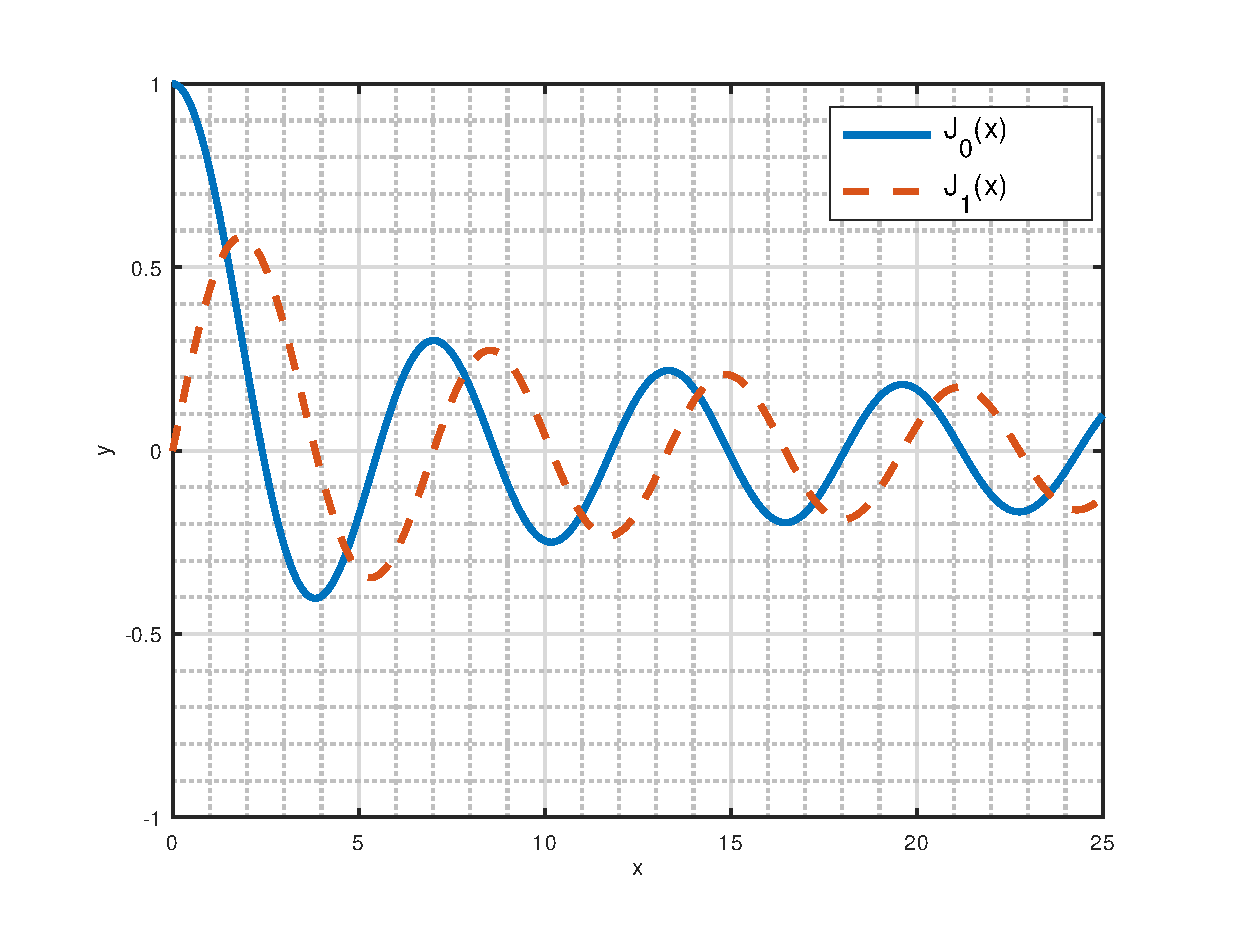
\includegraphics[scale=0.52]{bessel}\vspace{-2mm}
\caption[]{\enskip Bessel functions $J_0(x)$ and $J_1(x)$}
\label{fig:bessel}
\end{figure}
\newpage
\startexercises\label{sec9dot4}
{\small
\probs{A}
\par\noindent For Exercises 1-8 find the interval of convergence of the given
power series.
\begin{enumerate}[item-label={\bfseries \arabic*.}]
\begin{multicols}{4}
 \item $\bigsum{n = 1}{\infty}~ \dfrac{n x^n}{(n + 1)^2}$
 \item $\bigsum{n = 1}{\infty}~ \dfrac{n x^n}{2^n}$
 \item $\bigsum{n = 1}{\infty}~ n^2 \,(x - 2)^n\vphantom{\dfrac{(x + 4)^n}{2^n}}$
 \item $\bigsum{n = 0}{\infty}~ \dfrac{(x + 4)^n}{2^n}$
\end{multicols}
\begin{multicols}{4}
 \item $\bigsum{n = 1}{\infty}~ \dfrac{(x + 1)^n}{n^n}$
 \item $\bigsum{n = 1}{\infty}~ n^n \,x^n\vphantom{\dfrac{(x + 1)^n}{n^n}}$
 \item $\bigsum{n = 0}{\infty}~ (-1)^n\,x^n\vphantom{\dfrac{(x + 1)^n}{n^n}}$
 \item $\bigsum{n = 1}{\infty}~ \dfrac{n x^n}{n + 1}$
\end{multicols}
 \item Note that power series of the form $\sum_{n=0}^{\infty} a_n x^n$ have an
  issue at $x=0$ when $n=0$: $0^0$ is an indeterminate form---it can equal
  anything (or nothing). What value has it implicitly been assigned so far?
  What would be the technically correct way to write the series
  $\sum_{n=0}^{\infty} a_n x^n$ so that this issue goes away?
 \item Show that
\[
\sum_{n=1}^{\infty}\,n\,x^n ~=~ \frac{x}{(1-x)^2} \quad\text{for $~-1<x<1$.}
\]
 \item Write the following infinite series as a rational number:
\[
\frac{1}{10} \;+\; \frac{2}{100} \;+\; \frac{3}{1000} \;+\; \frac{4}{10000}
\;+\; \cdots
\]
\suspend{enumerate}
\probs{B}
\resume{enumerate}[item-label={{[\bfseries \arabic*.]}}]
 \item Differentiating term by term, verify that the Bessel function $J_0(x)$
  satisfies Bessel's equation (see equation (\ref{eqn:besseldiffeq})).
 \item Show that for all $m \ge 1$ the Bessel functions $J_m(x)$ converge for
  all $x$.
 \item For all $m \ge 1$ verify that the Bessel functions $J_m(x)$ satisfy the
  general Bessel equation of order $m$
  (see equation(\ref{eqn:besseldiffeqgen})).
 \item\label{exer:besselderiv} For the Bessel functions $J_0(x)$ and $J_1(x)$
  show that:
\begin{enumerate}[item-label={\bfseries (\alph*)}]
\item $\Ddx\,(x\,J_1(x)) ~=~ x\,J_0(x)$
\item $\int J_0(x)\,J_1(x)~\dx ~=~ -\frac{1}{2}\,J_0^2(x)$
\item $\int x\,J_0(x)\,J_1(x)~\dx ~=~ -\frac{1}{2}\,x\,J_0^2(x) ~+~
\frac{1}{2}\,\int J_0^2(x)~\dx$
\item For all integers $n\ge 2$,
\[
\int x^n\,J_0(x)~\dx ~=~ x^n\,J_1(x) ~+~ (n-1)\,x^{n-1}\,J_0(x) ~-~
(n-1)^2\,\int x^{n-2}\,J_0(x)~\dx ~.
\]
\emph{(Hint: Use part (a) and integration by parts twice.)}
\end{enumerate}
 \item For all integers $m\ge 2$ show that the Bessel functions $J_m(x)$
  satisfy the relations:
\begin{enumerate}[item-label={\bfseries (\alph*)}]
\item $m\,J_m(x) ~+~ x\,J_m'(x) ~=~ x\,J_{m-1}(x)$
\item $J_{m-1}(x) ~-~ J_{m+1}(x) ~=~ 2J_{m}'(x)$
\end{enumerate}
 \item Use long division to obtain the first three terms of
  $\frac{1}{x J_0^2(x)}$, then integrate term by term to show that
\[
J_0(x)\,\int \frac{\dx}{x J_0^2(x)} ~=~ J_0(x)\,\cdot\,\ln\,x ~+~ \frac{x^2}{4}
~-~ \frac{3x^4}{128} ~+~ \cdots ~.
\]
This function is a \emph{Bessel function of the second kind} and is another
solution of Bessel's equation.
\end{enumerate}
}
\newpage
%Begin Section 9.5
\section{Taylor's Series}
In the previous section a few functions, e.g. $f(x) = \frac{1}{1-x}$, turned out
to be the sum of a power series. This section will discuss a general method for
representing a function as a power series, called a\index{Taylor's series}
\textbf{Taylor's series}.\footnote{Named after English mathematician Brook
Taylor (1685-1731), though such series were known to others (e.g. James Gregory,
Johann Bernoulli) before Taylor.} Suppose that a function $f(x)$ can be written
as
\[
f(x) ~=~ \sum_{n=0}^{\infty}\,a_n\,(x-c)^n
\]
either for all $x$ or for $\abs{x-c} < R$, for some $R>0$. Then $f(c) = a_0$,
and differentiating term by term yields\index{Taylor's formula}
\begin{alignat*}{4}
f'(x) ~&=~ \sum_{n=1}^{\infty}\,n\,a_n\,(x-c)^{n-1} &&\Rightarrow \quad
           &f'(c) ~&=~ 1\,\cdot\,a_1\\[2pt]
f''(x) ~&=~ \sum_{n=2}^{\infty}\,n\,(n-1)\,a_n\,(x-c)^{n-2} &&\Rightarrow \quad
           &f''(c) ~&=~ 2\,\cdot\,1\,\cdot\,a_2\\[2pt]
f'''(x) ~&=~ \sum_{n=3}^{\infty}\,n\,(n-1)\,(n-2)\,a_n\,(x-c)^{n-3} &&\Rightarrow \quad
           &f'''(c) ~&=~ 3\,\cdot\,2\,\cdot\,1\,\cdot\,a_3\\
&\cdots & {} & {} & {} &\cdots\\
f^{(k)}(x) ~&=~ \sum_{n=k}^{\infty}\,n\,(n-1)\,(n-2)\,\cdots\,(n-k+1)\,a_n\,(x-c)^{n-k}
\quad &&\Rightarrow \quad &f^{(k)}(c) ~&=~ k !\;a_k
\end{alignat*}
so that in general (since $f^{(0)}(x) = f(x)$ and $0 ! = 1$):
\begin{equation}\label{eqn:taylorcoeff}
a_n ~=~ \frac{f^{(n)}(c)}{n !} \quad\text{for $~n \ge 0$}
\end{equation}
These $\seq{a_n}$ are the \textbf{Taylor's series coefficients} of $f(x)$ at
$x=c$. The full power series representation of $f(x)$ can now be stated:

\statethm{thm:taylor}{\textbf{Taylor's formula}: If $f(x)$ has a power series
representation in powers of $x-c$, where $x=c$ is inside the interval of
convergence, then that representation is unique in that interval and is given by
\begin{equation}\label{eqn:taylorseries}
f(x) ~=~ \bigsum{n=0}{\infty}~ \frac{f^{(n)}(c)}{n !}\,(x-c)^n
\end{equation}
for all $x$ in the interval. This is the \textbf{Taylor's series} for $f(x)$
about $x=c$.}
\newpage
\begin{exmp}\label{exmp:taylorexp}
\noindent Find the Taylor's series for $f(x)=e^x$ about $x=0$.\vspace{1mm}
\par\noindent\emph{Solution:} Since $\ddx\,(e^x) = e^x$, then for all $n\ge 0$,
\[
f^{(n)}(x) ~=~ e^x \quad\Rightarrow\quad f^{(n)}(0) ~=~ e^0 ~=~ 1 ~.
\]
Thus, by Taylor's formula with $c=0$:\footnote{The special case of $c=0$ in
Taylor's formula yields what is sometimes called the \emph{Maclaurin's series}
for $f(x)$,\index{Maclaurin's series} though that terminology is typically not
used in fields of study outside mathematics.}
\begin{align*}
e^x ~&=~ \bigsum{n=0}{\infty}~ \frac{f^{(n)}(0)}{n !}\,x^n ~=~
\bigsum{n=0}{\infty}~ \frac{x^n}{n !}\\
&=~ 1 ~+~ x ~+~ \frac{x^2}{2 !} ~+~ \frac{x^3}{3 !} ~+~ \frac{x^4}{4 !} ~+~
\frac{x^5}{5 !} ~+~ \cdots
\end{align*}
For what $x$ is this Taylor's series valid? Recall that Example
\ref{exmp:expseries} showed the interval of convergence is all of $\Reals$. Thus
the above Taylor's series holds for all $x$.
\end{exmp}
\divider
\vspace{2mm}

Before continuing, you might be wondering why you should even bother with
finding the Taylor's series---after all, in the above example why replace a
simple function like $e^x$ by a far more complicated expression? One reason is
that it often helps simplify some computations, especially in integrals. The
idea is to use only a few terms in the series, i.e. a polynomial, as an
approximation, since polynomials are generally easier to work with. Perhaps
surprisingly, in many practical applications no more than two terms are needed,
and often only one.

For example, using only the first two terms of the Taylor's series for
$e^x$ in Example \ref{exmp:taylorexp}, $e^x \approx 1 + x$ is a good
approximation when $x$ is close to 0 (i.e. $\abs{x} \ll 1$). Using more terms
does not necessarily help---for $\abs{x} \ll 1$ and $n>1$, $x^n$ will be
effectively 0. So the added complexity would not make the approximation
significantly better.

\begin{exmp}\label{exmp:approxe}
\noindent The energy density $E$ of electromagnetic radiation at wavelength
$\lambda$ from a black-body at temperature $T$ degrees Kelvin is given by
\emph{Planck's Law} of black-body radiation,
\[
 E(\lambda) ~=~ \frac{8\pi h c}{\lambda^5 (e^{hc/\lambda kT} - 1)}
\]
where $h$ is Planck's constant, $c$ is the speed of light, and $k$ is Boltzmann's
constant. Show that for $\lambda \gg 1$:
\[
E(\lambda) ~\approx~ \frac{8\pi kT}{\lambda^4}
\]
\par\noindent\emph{Solution:} Since $e^x ~\approx~ 1 + x\;$ for $\abs{x} \ll 1$
by the Taylor series for $e^x$, let $x = hc/\lambda kT$. Then $x \ll 1$ and so
\[
E(\lambda) ~=~ \frac{8\pi h c}{\lambda^5 (e^{hc/\lambda kT} - 1)} ~\approx~
 \frac{8\pi h c}{\lambda^5 \left(\left(1 + \frac{hc}{\lambda kT}\right) - 1\right)}
~\approx~  \frac{8\pi h c}{\lambda^5 \frac{hc}{\lambda kT}} ~\approx~
\frac{8\pi kT}{\lambda^4}
\]
\end{exmp}
\divider
\newpage
\begin{exmp}\label{exmp:taylorsin}
\noindent Find the Taylor's series for $f(x)=\sin\,x$ about $x=0$.\vspace{1mm}
\par\noindent\emph{Solution:} The derivatives of $f(x)=\sin\,x$ repeat every
four derivatives:
\[
f(x) ~=~ \sin\,x \quad,\quad
f'(x) ~=~ \cos\,x \quad,\quad
f''(x) ~=~ -\sin\,x \quad,\quad
f'''(x) ~=~ -\cos\,x \quad,\quad
f^{(4)}(x) ~=~ \sin\,x
\]
So at $x=0$:
\[
f(0) ~=~ 0 \quad,\quad
f'(x) ~=~ 1 \quad,\quad
f''(x) ~=~ 0 \quad,\quad
f'''(x) ~=~ -1 \quad,\quad
f^{(4)}(x) ~=~ 0
\]
So for $n\ge 0$,
\[
f^{(n)}(0) ~=~ \begin{cases} ~0 & \text{if $~n$ is even,}\\
~1 & \text{if $~n=1,5,9,\ldots$,}\\~-1 & \text{if $~n=3,7,11,\ldots$.}\end{cases}
\]
Thus, by Taylor's formula with $c=0$
\begin{align*}
\sin\,x ~&=~ \bigsum{n=0}{\infty}~ \frac{f^{(n)}(0)}{n !}\,x^n\\[4pt]
&=~ x ~-~ \frac{x^3}{3 !} ~+~ \frac{x^5}{5 !} ~-~ \frac{x^7}{7 !} ~+~
\frac{x^9}{9 !} ~-~ \cdots\\[4pt]
&=~ \bigsum{n=0}{\infty}~ (-1)^{n}\,\frac{x^{2n+1}}{(2n+1) !}
\end{align*}
By the Ratio Test this series converges for all $x$, since for any fixed $x$,
\[
r(x) ~=~ \lim_{n \to \infty} \;\left|\dfrac{(-1)^{n+1}\,\dfrac{x^{2n+3}}{(2n+3) !}}
{(-1)^{n}\,\dfrac{x^{2n+1}}{(2n+1) !}}\right| ~=~
x^2 \;\cdot\; \lim_{n \to \infty} \;\Biggl|\frac{1}{(2n+3)\,(2n+2)}\Biggr| ~=~ 0 ~<~ 1 ~.
\]
\end{exmp}
\begin{exmp}\label{exmp:taylorcos}
\noindent Find the Taylor's series for $f(x)=\cos\,x$ about $x=0$.\vspace{1mm}
\par\noindent\emph{Solution:} The Taylor's series can be found using the same
procedure as in Example \ref{exmp:taylorsin}, but it is simpler to just
differentiate the Taylor's series for $\sin\,x$ term by term for all $x$:
\begin{align*}
\cos\,x ~&=~ \ddx\,(\sin\,x) ~=~
\ddx\,\left(x ~-~ \frac{x^3}{3 !} ~+~ \frac{x^5}{5 !} ~-~ \frac{x^7}{7 !} ~+~
\frac{x^9}{9 !} ~-~ \cdots\right)\\[4pt]
&=~ 1 ~-~ \frac{x^2}{2 !} ~+~ \frac{x^4}{4 !} ~-~ \frac{x^6}{6 !} ~+~
\frac{x^8}{8 !} ~-~ \cdots\\[4pt]
&=~ \bigsum{n=0}{\infty}~ (-1)^{n}\,\frac{x^{2n}}{(2n) !}
\end{align*}
Since the Taylor's series for $\sin\,x$ converges for all $x$ then so does its
derivative. Thus the Taylor's series for $\cos\,x$ converges for all
$x$.\\Notice that the Taylor's series for $\cos\,x$ has only even powers of $x$, while
the series for $\sin\,x$ has only odd powers of $x$. This makes sense since
$\cos\,x$ and $\sin\,x$ are even and odd functions, respectively.
\end{exmp}
\divider
\newpage
\begin{exmp}\label{exmp:taylorlog}
\noindent The function $\ln\,x$ is not defined at $x=0$ and hence has no
Taylor's series about $x=0$. Instead, find the Taylor's series for
$f(x)=\ln\,(1+x)$ about $x=0$.\vspace{1mm}
\par\noindent\emph{Solution:} Take successive derivatives:
\[
f(x) ~=~ \ln\,(1+x) \quad,\quad
f'(x) ~=~ \frac{1}{1+x} \quad,\quad
f''(x) ~=~ -\frac{1}{(1+x)^2} \quad,\quad
f'''(x) ~=~ \frac{1 \,\cdot\, 2}{(1+x)^3} \quad,\quad
f^{(4)}(x) ~=~ -\frac{1 \,\cdot\, 2 \,\cdot\, 3}{(1+x)^4}
\]
So $f(0)=0$ and for $n\ge 1$:
\[
f^{(n)}(x) ~=~ (-1)^{n-1}\,\frac{(n-1) !}{(1+x)^n} \quad\Rightarrow\quad
f^{(n)}(0) ~=~ (-1)^{n-1}\,(n-1) !
\]
Thus, by Taylor's formula,
\begin{align*}
\ln\,(1+x) ~&=~ \bigsum{n=0}{\infty}~ \frac{f^{(n)}(0)}{n !}\,x^n ~=~
\bigsum{n=1}{\infty}~ (-1)^{n-1}\,\frac{(n-1) !\,x^{n}}{n !}\\[4pt]
&=~ \bigsum{n=1}{\infty}~ (-1)^{n-1}\,\frac{x^{n}}{n}\\[4pt]
&=~ x ~-~ \frac{x^2}{2} ~+~ \frac{x^3}{3} ~-~ \frac{x^4}{4} ~+~
\frac{x^5}{5} ~-~ \cdots
\end{align*}
Use the Ratio Test to find the interval of convergence:
\[
r(x) ~=~ \lim_{n \to \infty} \;\left|\dfrac{(-1)^{n}\,\dfrac{x^{n+1}}{n+1}}
{(-1)^{n-1}\,\dfrac{x^{n}}{n}}\right| ~=~
\abs{x} \;\cdot\; \lim_{n \to \infty} \;\Biggl|\frac{n}{n+1}\Biggr| ~=~
\abs{x} \,\cdot\, 1 ~=~ \abs{x}
\]
So the series converges when $\abs{x} < 1$. Check the cases $r(x)=\abs{x}=1$
individually. For $x=1$ the series is the alternating harmonic series
$\sum_{n=1} \frac{(-1)^{n-1}}{n}$, which converges. For $x=-1$ the series is
$-\sum_{n=1} \frac{1}{n}$, the negative of the harmonic series, which diverges.
Thus, the series converges for $-1<x\le 1$.
\end{exmp}
\begin{exmp}\label{exmp:taylorexp2}
\noindent Find the Taylor's series for $f(x)=e^{x^2}$ about $x=0$.\vspace{1mm}
\par\noindent\emph{Solution:} The Taylor's series can be found using the same
procedure as in Example \ref{exmp:taylorexp}, but it is simpler to just
replace each occurrence of $x$ in the Taylor's series for $e^x$ by $x^2$ (since
the series for $e^x$ converges for all $x$). In
other words, make the substitution $u=x^2$ in the Taylor's series for $e^u$
about $u=0$:
\begin{align*}
e^u ~&=~ \bigsum{n=0}{\infty}~ \frac{u^n}{n !}\\[4pt]
e^{x^2} ~&=~ \bigsum{n=0}{\infty}~ \frac{(x^2)^n}{n !} ~=~
\bigsum{n=0}{\infty}~ \frac{x^{2n}}{n !}\\[4pt]
&=~ 1 ~+~ x^2 ~+~ \frac{x^4}{2 !} ~+~ \frac{x^6}{3 !} ~+~
\frac{x^8}{4 !} ~+~ \frac{x^{10}}{5 !} ~+~ \cdots
\end{align*}
\end{exmp}
\divider
\newpage
\noindent Define the \textbf{$\bm{n}$-th degree Taylor polynomial} $P_n(x)$ for
a function $f(x)$ about $x=c$ by\index{Taylor polynomial}
\begin{align*}
P_n(x) ~&=~ \bigsum{k=0}{n}~ \frac{f^{(k)}(c)}{k !}\,(x-c)^k\\
&=~ f(c) ~+~ \frac{f'(c)}{1 !}\,(x-c) ~+~ \frac{f''(c)}{2 !}\,(x-c)^2 ~+~ \cdots ~+~
\frac{f^{(n)}(c)}{n !}\,(x-c)^n
\end{align*}
for $x$ in the interval of convergence for the full Taylor's series. In other
words, $P_n(x)$ is the $n$-th partial sum of the Taylor's series. Since some of
the coefficients could be zero, $P_n(x)$ is a polynomial of degree at most
$n$. Thus, $P_n(x) = O(x^n)$. For that reason $P_n(x)$ is
sometimes called the \textbf{$\bm{O(x^n)}$ approximation} to $f(x)$.

Figure \ref{fig:sinetaylor} shows a comparison of $\sin\,x$ with a few
of its approximations:\vspace{-3mm}

\begin{figure}[ht]
\centering
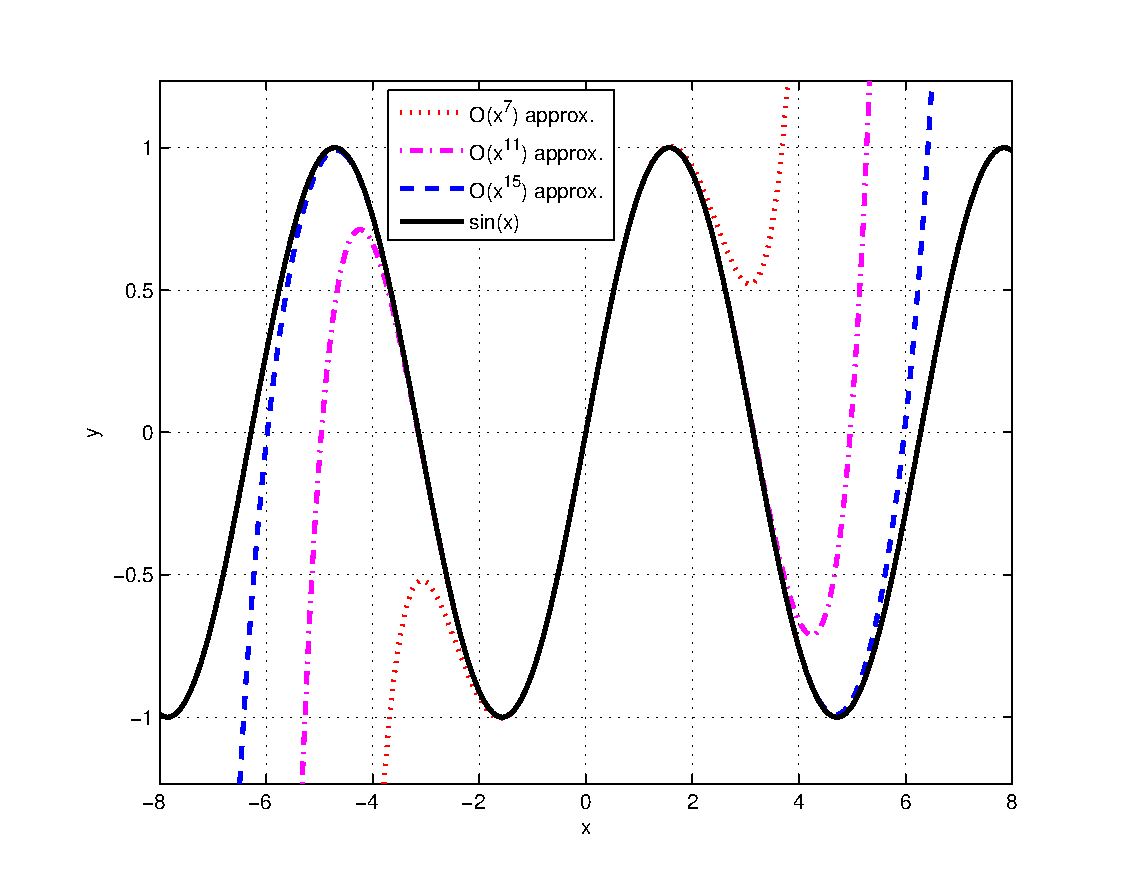
\includegraphics[scale=0.70]{sinetaylor}\vspace{-2mm}
\caption[]{\enskip $\sin\,x$ and Taylor's series approximations}
\label{fig:sinetaylor}
\end{figure}

As you can see, the Taylor polynomials of degree 7, 11 and 15 are all good
approximations over the interval $\ival{-2}{2}$, with the $O(x^{15})$
approximation still being fairly good over $\ival{-6}{6}$. Clearly those
approximations all become poor quite quickly for $\abs{x} > 6$; they approach
$\pm\infty$, unlike $\sin\,x$.

The following theorem shows how to measure the accuracy of the
approximations:
\newpage
\statethm{thm:taylorremainder}{\textbf{Remainder Theorem}:\footnotemark If
$P_n(x)$ is the $n$-th degree Taylor polynomial about $x=c$ for a function
$f(x)$ in some interval containing $x=c$, then for all $x$ in that interval,
\begin{equation}\label{eqn:taylorremainder}
f(x) ~=~ P_n(x) ~+~ R_n(x) ~,
\end{equation}
where
\begin{equation}\label{eqn:taylorrem1}
R_n(x) ~=~ \frac{f^{(n+1)}(c +\theta (x-c))}{(n+1) !}\,(x-c)^{n+1}
\end{equation}
for some number $\theta$ between 0 and 1. Alternatively,
\begin{equation}\label{eqn:taylorrem2}
R_n(x) ~=~ \frac{1}{n !}\,\int_c^x (x-t)^{n}\,f^{(n+1)}(t)~\dt ~.
\end{equation}
}\footnotetext{For a proof see
pp.171-172 in \textsc{Klambauer, G.}, \emph{Aspects of Calculus}, New York:
Springer-Verlag, 1986.}\index{Taylor's series!Remainder Theorem}

Since the number $\theta$ is unknown in equation (\ref{eqn:taylorrem1}),
usually only an upper bound on the remainder $R_n(x)$ can be found by that
formula. For practical purposes formula (\ref{eqn:taylorrem2}) for $R_n(x)$
might be easier to use (via numerical integration).

A common misconception is that hand-held calculators use Taylor's series to
compute values of functions like $\sin\,x$, $\cos\,x$, $e^x$, etc. However, that
is typically well beyond their capability, especially for large values of
$x$---far too
many terms would be required. Instead, many calculators use an algorithm called
CORDIC\footnote{See Ch.7 in \textsc{Schmid, H.}, \emph{Decimal Computation},
New York: John Wiley \& Sons, Inc., 1974.}
(Coordinate Rotation Digital Computer), and---perhaps\index{CORDIC}
surprisingly---lookup tables. CORDIC uses the computationally
inexpensive operation of bit-shifting to translate large input values into a
smaller range, then uses tables stored in memory for values in that range, along
with interpolation for numbers between those in the tables.\footnote{To see how
inaccurate calculators can be, compute $\tan (355/226)$ in radian mode on a
calculator. The true value to 3 decimal places is $-7497258.185$, but few
calculators produce an answer close to that.}

\divider
\vspace{2mm}
\startexercises\label{sec9dot5}
{\small
\probs{A}
\par\noindent For Exercises 1-9 write out the first three nonzero terms in the
Taylor's series for the given function $f(x)$ about the given value $c$. You may
use any method you like.
\begin{enumerate}[item-label={\bfseries \arabic*.}]
\begin{multicols}{3}
 \item $f(x) = \sin\,x$ ; $c = \pi/2$
 \item $f(x) = \sinh\,x$ ; $c = 0$
 \item $f(x) = \cosh\,x$ ; $c = 0$
\end{multicols}
\begin{multicols}{3}
 \item\label{exer:taylortan} $f(x) = \tan\,x$ ; $c = 0$
 \item\label{exer:taylortanh} $f(x) = \tanh\,x$ ; $c = 0$
 \item $f(x) = \sec\,x$ ; $c = 0$
\end{multicols}
\begin{multicols}{3}
 \item\label{exer:tayloratan} $f(x) = \dfrac{1}{1 +x^2}$ ; $c = 0$
 \item $f(x) = \dfrac{1}{1 + x^2}$ ; $c = 1$
 \item\label{exer:taylorsq} $f(x) = \sqrt{1 + x^2}$ ; $c = 0\vphantom{\dfrac{1}{x^2 ~+~ 1}}$
\end{multicols}
 \item Use Example \ref{exmp:seriesderivxn} from Section 9.4 to write out the
  first three nonzero terms in the Taylor's series for
  $f(x) = \frac{1}{(1 - x)^3}$ about $x=0$.
 \item Use the derivative of the Taylor's series for $\sqrt{1 + x^2}$ from
  Exercise \ref{exer:taylorsq} to write out the first three nonzero terms in the
  Taylor's series for $f(x) ~=~ \frac{x^2}{\sqrt{1 + x^2}}$ about $x=0$.
\suspend{enumerate}
\par\noindent For Exercises 12-15 replace the function $f(x)$ by its Taylor's
 series about $x=0$ to evaluate the given indefinite integral $\int f(x) \;\dx$
 (up to the first three nonzero terms in the series).
\resume{enumerate}[item-label={{[\bfseries \arabic*.]}}]
\begin{multicols}{4}
 \item $\displaystyle\int \frac{\sin\,x}{x}~\dx$
 \item $\displaystyle\int \cos\,(x^2)~\dx\vphantom{\displaystyle\int \frac{\sin\,x}{x}}$
 \item $\displaystyle\int e^{-x^2}~\dx\vphantom{\displaystyle\int \frac{\sin\,x}{x}}$
 \item $\displaystyle\int \sqrt{1+x^6}~\dx\vphantom{\displaystyle\int \frac{\sin\,x}{x}}$
\end{multicols}
 \item\label{exer:atanpi} Use $\ddx\,(\tan^{-1} x) = \frac{1}{1+x^2}$ along with
  Exercise \ref{exer:tayloratan} to find the Taylor's series for
  $f(x)=\tan^{-1} x$ about $x=0$, along with its interval of convergence.
 \item Use Exercise \ref{exer:atanpi} to show that
\[
\pi ~=~ 4\,\left(1 \;-\; \frac{1}{3} \;+\; \frac{1}{5} \;-\; \frac{1}{7}
\;+\; \cdots \right) ~.
\]
 \item Use the first three nonzero terms in the Taylor's series about $x=0$ for
 $e^{-x^2/2}$ to evaluate the definite integral
 \begin{displaymath}
  \int_{-1}^1 ~\frac{1}{\sqrt{2\pi}} \,e^{-x^2/2}~\dx \quad .
 \end{displaymath}
  Note: The actual value (rounded to 4 decimal places) is 0.6826.
 \item Recall that the surface area $S$ of the solid obtained by revolving the
  curve $y = x^2$ around the $x$-axis between $x = 0$ and $x = 2$ is given by
  the integral
 \begin{displaymath}
  S ~=~ \int_0^2 ~2 \pi x^2 \,\sqrt{1 \;+\; 4x^2}~\dx \quad .
 \end{displaymath}
 The exact value of the integral rounded to 3 decimal places is $S = 53.226$.
 Use the first two nonzero terms in the Taylor's series for $\sqrt{1 + 4x^2}$
 about $x=0$ to approximate the integral. How close is this approximation to the
 actual value? Does the approximation become better if you use the first three
 nonzero terms in the Taylor's series? Justify your answer.
 \item The tangential component of a space shuttle's velocity during reentry is
 approximately
\[
 v(t) ~=~ v_c \,\tanh\,\left( \frac{g}{v_c} t ~+~
 \tanh^{-1} \left(\frac{v_0}{v_c}\right) \right)
\]
  where $v_0$ is the velocity at time $t=0$ and $v_c$ is the terminal velocity.
  If $\tanh^{-1} \left(\frac{v_0}{v_c}\right) = \frac{1}{2}$ then show that
  $v(t) \approx gt + \frac{1}{2}v_c$.
 \item The velocity of a water wave of length $L$ in water of depth $h$
 satisfies the equation
 $v^2 = \frac{gL}{2\pi} \tanh \left( \frac{2\pi h}{L}\right)$. Show that
 $v \approx \sqrt{gh}$.
 \item A disk of radius $a$ has a charge of constant density $\sigma$. A point
 $P$ lies at a distance $r$ directly above the disk. The
 \emph{electrical potential} $V$ at point $P$ is given by
 $V = 2\pi\sigma(\sqrt{r^2 + a^2} - r)$. Show that
 $V \approx \frac{\pi a^2 \sigma}{r}$ for large $r$ (i.e. $r \gg 1$).
 \item The fifth-degree \emph{Pad\'{e} approximation} uses rational functions to
  approximate $\tanh\,x$:\index{Pad\'{e} approximation}
\[
 \tanh\,x ~\approx~ \frac{x^5 + 105x^3 + 945x}{15x^4 + 420x^2 + 945}
\]
 Compare the values of the Pad\'{e} approximation and the fifth-degree Taylor's
 series approximation from Exercise \ref{exer:taylortanh}, evaluated at $x=1$.
 Which is better? The actual value of $\tanh (1)$ is 0.7615941559558. How do
 the two approximations compare at $x=2$?
\end{enumerate}


}
